\documentclass[a4paper,fleqn]{cas-sc}

\usepackage[authoryear]{natbib}
\usepackage{graphicx} 
\usepackage{float}
\usepackage{algorithm}  
\usepackage{algpseudocode}
\usepackage{color}
\usepackage{setspace}
\usepackage[nomarkers,figuresonly]{endfloat}

\usepackage{dirtree}

\newcommand{\colorComments}{black} 
 
%%%Author definitions
\def\tsc#1{\csdef{#1}{\textsc{\lowercase{#1}}\xspace}}
\tsc{MS}
\tsc{AFO}
%%%

\usepackage{lineno}
\linenumbers 

\begin{document}
\let\WriteBookmarks\relax
\def\floatpagepagefraction{1}
\def\textpagefraction{.001}
\shorttitle{formikoj - Flexible geophysical data processing}
\shortauthors{Steiner and Flores Orozco}

\title [mode = title]{formikoj: A flexible library for data management and processing in geophysics - Application for seismic refraction data}


\author[1]{Matthias Steiner}[type=editor,
                        auid=000,bioid=1,orcid=0000-0002-3595-3616]
\cormark[1]
\cortext[1]{Corresponding author}
\credit{Conceptualization and implementation of the library, creating the figures, preparation of the manuscript}

\author[1]{Adrián {Flores Orozco}}[orcid=0000-0003-0905-3718] 
\credit{Conceptualization of the library, preparation of the manuscript}

\address[1]{Research Unit Geophysics, Department of Geodesy and Geoinformation, TU Wien}

\begin{abstract}
We introduce here the open-source library formikoj, which provides a flexible framework for managing and processing geophysical data collected in environmental and engineering investigations. To account for the substantial changes regarding the market shares of operating systems within the last two decades, the library is specifically implemented and tested for cross-plattform usage.
We illustrate the applicability of the formikoj library to forward-model seismic refraction waveform data with the \texttt{SeismicWaveformModeler} based on a custom subsurface model and survey geometry. 
Moreover, we present two case studies from seismic refraction tomography field measurements to exemplify the wide range of possibilities provided by the formikoj library for the processing of real data. In particular, we explore different visualization of the seismic traveltime readings to enhance their consistency prior to the inversion. 
The low-level access provided by our library aims at giving the users the possibility to implement particular modeling, visualization and processing tools specifically designed for their objectives or other geophysical methods.
\end{abstract}
 
\begin{coverletter}

Dear Editors-in-Chief,
\newline
 
we are submitting our manuscript "formikoj: A flexible library for data management and processing in geophysics - Application for seismic refraction data", which we consider is a suitable contribution for Computers \& Geosciences. We confirm that the submission follows all the requirements and includes all the items of the submission checklist.  
\newline
 
The manuscript presents the open-source python library formikoj for managing and processing geophysical data collected in environmental and engineering investigations. formikoj was specifically implemented for multi-platform usage to allow the efficient collaboration and exchange of data between different partners in research projects and academia. In this regard, we believe that this library aids in providing reproducible data and results as well as establishing and maintaining good research practices. Accordingly, we consider this manuscript relevant to the audience of Computers \& Geosciences, and in general for geoscientists and practitioners working with geophysical methods.
\newline

We provide the source codes in a public repository with details listed in the section "Code availability".
\newline

We look forward to your decision.
\newline

Yours sincerely,
\newline

Matthias Steiner and Adrián Flores Orozco

Research Unit Geophysics, Department of Geodesy and Geoinformation, TU Wien; matthias.steiner@geo.tuwien.ac.at
\newline

\end{coverletter}
 
\begin{highlights}
\item flexible open-source and cross-platform library for managing and processing of geophysical data
\item possibility to be deployed for different geophysical methods and/or instruments
\item application for the modeling and processing of seismic refraction datasets
\item applicable for seismic refraction data collected in 2D and 3D survey geometries
\item easily scalable for custom requirements
\end{highlights}

\begin{keywords}
geophysical data processing \sep seismic refraction \sep first break picking \sep seismic waveform modeling \sep cross-platform application \sep geophysical python library \sep flexible open-source librarys \sep wave based methods
\end{keywords}

\maketitle 

\printcredits

\doublespacing

\section{Introduction}
\label{intro}

The acquisition of spatially quasi-continuous data in a non-invasive manner renders geophysical methods suitable for engineering and environmental investigations \citep[e.g.,][]{parsekian2015, nguyen2018, romero2019}.
%Several studies have demonstrated the successful application of geophysical methods, for instance, to evaluate groundwater remediation techniques \citep[e.g.,][]{floresorozco2015}, as well as for the investigation of landfills \citep[e.g.,][]{nguyen2018, steiner2022}, soil structure \citep[e.g.,][]{romero2019}, or the critical zone \citep[e.g.,][]{parsekian2015}. 
However, the processing of geophysical data often relies on commercial software solutions and the associated licensing costs might render their use prohibitively expensive, which might be the case for academic projects or institutions.
The most popular packages are Res2DInv\footnote{https://www.geometrics.com/software/res2dinv/, last accessed on \today} for electrical methods, Halliburton Landmark SeisSpace ProMAX\footnote{https://www.landmark.solutions/SeisSpace-ProMAX, last accessed on \today} or ParkSeis \footnote{https://www.parkseismic.com/parkseis/, last accessed on \today} for seismic methods, or ReflexW\footnote{https://www.sandmeier-geo.de/reflexw.html, last accessed on \today} for ground-penetrating radar and seismic methods.
%, or the Zond\footnote{http://zond-geo.com/english/zond-software/, last accessed on \today} processing tools for various geophysical methods including seismic, gravimetric and electromagnetic data. 
A common limitation of the aforementioned software solutions refers to their specific platform requirements mainly related to the type and version of the operating system; moreover, the possibility to adapt the code are limited if possible at all. Considering the substantial changes regarding the market shares of operating systems within the last two decades, platform-specific software packages are becoming particularly obstructive for academic research and teaching.
The increasing popularity of the Python programming language led to the development of various cross-platform open-source software packages for processing, modeling and inverting geophysical data. Available packages can focus on specific geophysical methods, for instance, ResIPy \citep{blanchy2020} for electrical data, GPRPy \citep{plattner2020} for ground-penetrating radar data, or ObsPy \citep{beyreuther2010} and Pyrocko \citep{heimann2017} for seismological data. Other packages provide frameworks for the inversion and permit the inclusion of forward models for different geophysical methods, e.g., SimPEG \citep{cockett2015}, Fatiando a Terra \citep{uieda2013} or pyGIMLi \citep{ruecker2017}. 

The seismic refraction tomography (SRT) is a standard technique in environmental and engineering applications. Often applied together with other geophysical methods, the SRT is routinely used, e.g., in 
%alpine and arctic 
permafrost studies \citep[e.g.,][]{draebing2016, steiner2021}, for the investigation of landfills \citep[e.g.,][]{nguyen2018, steiner2022}, or for hydrogeological characterizations \citep[e.g.,][]{buecker2021}. 
The market for seismic processing software has long been dominated by software packages designed for the processing of large datasets, e.g., associated to oil or gas exploration. 
Accordingly, these seismic processing solutions may not be suited for small-scale projects in environmental and engineering studies, or for teaching activities. 
ReflexW overcomes such limitations by providing processing tools specifically designed for near-surface investigations at substantially lower costs. In terms of licensing costs, 
%the developers of 
\citet{stockwell1999} went a step further by making the Seismic Unix framework available entirely free of charge; whereas \citet{guedes2022} recently presented RefraPy, a python processing tool for seismic refraction data. 
Implemented in python, RefraPy is potentially suitable for cross-platform usage, yet 
\citet{guedes2022} 
developed and tested 
%RefraPy 
solely for Windows operating systems. Moreover, RefraPy does not offer the possibility to generate synthetic seismic waveform data, as required for survey design, as well as teaching and interpretation purposes.

The formikoj library presented here is an open-source framework for creating synthetic datasets, as well as for managing and processing numerical and field data independently from the operating system and without licensing costs; thus, overcoming limitations associated to existing solutions. The design of the library follows the multi-method concept of pyGIMLi and SimPEG, which allows for the implementation of custom designed tools for different geophysical methods. 
The usage of transparent file formats, e.g., the unified data format (udf\footnote{http://resistivity.net/bert/data\_format.html, last accessed on \today}), and data management concepts (SQLite database) within the formikoj framework facilitates a simple data exchange between partners in research projects and academia, which is required to guarantee the repeatability of results and good research practices.
Considering the diverse applications of the SR method we demonstrate the applicability of the proposed library based on tools implemented within the formikoj framework for the modeling and processing seismic waveform data. 
In particular, we present here a series of illustrative use cases based on the formikoj library referring to (i) the modeling of synthetic seismic refraction (SR) waveform data, (ii) the processing of a 2D SR field dataset collected with a roll-along survey geometry, and (iii) the processing of a 3D SR field data set. 

\section{Design and structure of the \texttt{formikoj} library}

As illustrated in Figure~\ref{fig:scheme}, the formikoj library comprises a modeling and a processing module, which both rely on a common utilities module. The \texttt{DataModeler} and the \texttt{MethodManager} class provide the basis to add modeling or processing functionalities for specific geophysical methods. In particular, we present here the \texttt{SeismicWaveformModeler} and \texttt{SeismicRefractionManager} classes implemented within the formikoj framework, which aim at creating and processing seismic waveform data, respectively. Similar to RefraPy, these classes are built upon the functionalities of existing packages such as ObsPy for the processing of seismological data \citep[][]{beyreuther2010} and pyGIMLi for the modeling and inversion of different geophysical data \citep{ruecker2017}. Other important third party dependencies refer to NumPy \citep{harris2020} and Pandas \citep{mckinney2010} for general data handling, as well as matplotlib \citep{hunter2007} and PyVista \citep{sullivan2019} for data visualization. In the current version, we implemented and tested formikoj primarily on Linux machines, yet the library has been successfully used on all major operating systems, i.e., Linux, MacOS and Windows.

\begin{figure}
	\centering
	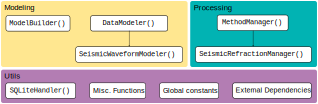
\includegraphics[width=.75\textwidth]{figures/package_structure}
	\caption{General architecture of the formikoj library comprising a utility, modeling and processing module. The base classes \texttt{DataModeler} and \texttt{MethodManager} can be used to build tools for specific geophysical methods, e.g., seismic refraction.}
	\label{fig:scheme}
\end{figure}

\subsection{Generation of seismic waveform data for synthetic subsurface models: The \texttt{SeismicWaveformModeler}}

The SR method exploits the ground motion recorded by sensors installed in the surface (e.g., geophones) to characterize the propagation of seismic waves generated at well known locations (i.e., shot stations). 
The visualization of the ground motion as function of time yields a so-called seismogram for each geophone position.
Accordingly, the \texttt{SeismicWaveformModeler} class provides a flexible way to generate synthetic seismic waveform data either in a python script, interactively in a jupyter notebook or an ipython shell. To create an instance of the class the path to the working directory is provided as parameter to the constructor:
\newline
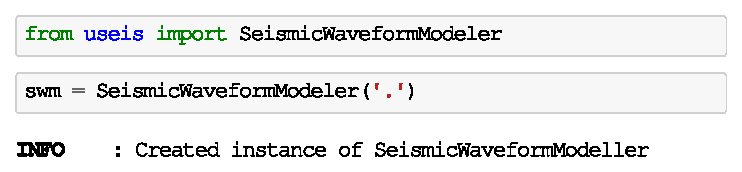
\includegraphics[width=.5\textwidth]{./figures/create_swm.pdf}
\newline
\\The working directory needs to contain a subdirectory \textit{in}, whereas the output directory \textit{out} will be created automatically:

\dirtree{%
.1 working\_directory.
.2 in.
.2 out.
}

\begin{table}[pos=h]
    \caption{Description of the information to be provided in the columns of a measurement scheme in csv format.}
    \centering
    \begin{tabular}{clcl}
        \toprule
        Column & \textbf{Content} & \textbf{Data type} & \textbf{Description} \\
        \midrule
        1 & x coordinate & float & Station x coordinate, e.g., given in (m) \\ 
        2 & y coordinate & float & Station y coordinate, e.g., given in (m) \\ 
        3 & z coordinate & float & Station z coordinate, e.g., given in (m) \\ 
        4 & Geophone & bool & 1 in case of a receiver station, 0 otherwise \\ 
        5 & Shot & bool & 1 in case of a shot station, 0 otherwise \\
        \bottomrule
    \end{tabular}
    \label{tab:scheme}
\end{table}
The required input files need to be provided via the subdirectory \textit{in} of the working directory. The key input file is the measurement scheme, which contains information regarding the distribution of the shot and geophone stations. If provided in the unified data format the measurement scheme is imported directly with pyGIMLi into a \texttt{DataContainer}. In case the measurement scheme is provided as a csv file the \texttt{SeismicWaveformModeler} reads the information and writes it to a pyGIMLi \texttt{DataContainer}. In the csv format the measurement scheme contains a single line for each station in the survey layout, where a station either hosts a geophone or a shot, or both (see Table~\ref{tab:scheme}). The values provided in each line need to be separated by a unique delimiter, and the file must not contain a header.

For the modeling of the seismic waveforms, the parameters for the base wavelet, the synthetic subsurface model and the resulting waveform datasets are provided (see Table~\ref{tab:config}) in a configuration file following the yaml format:
\newline
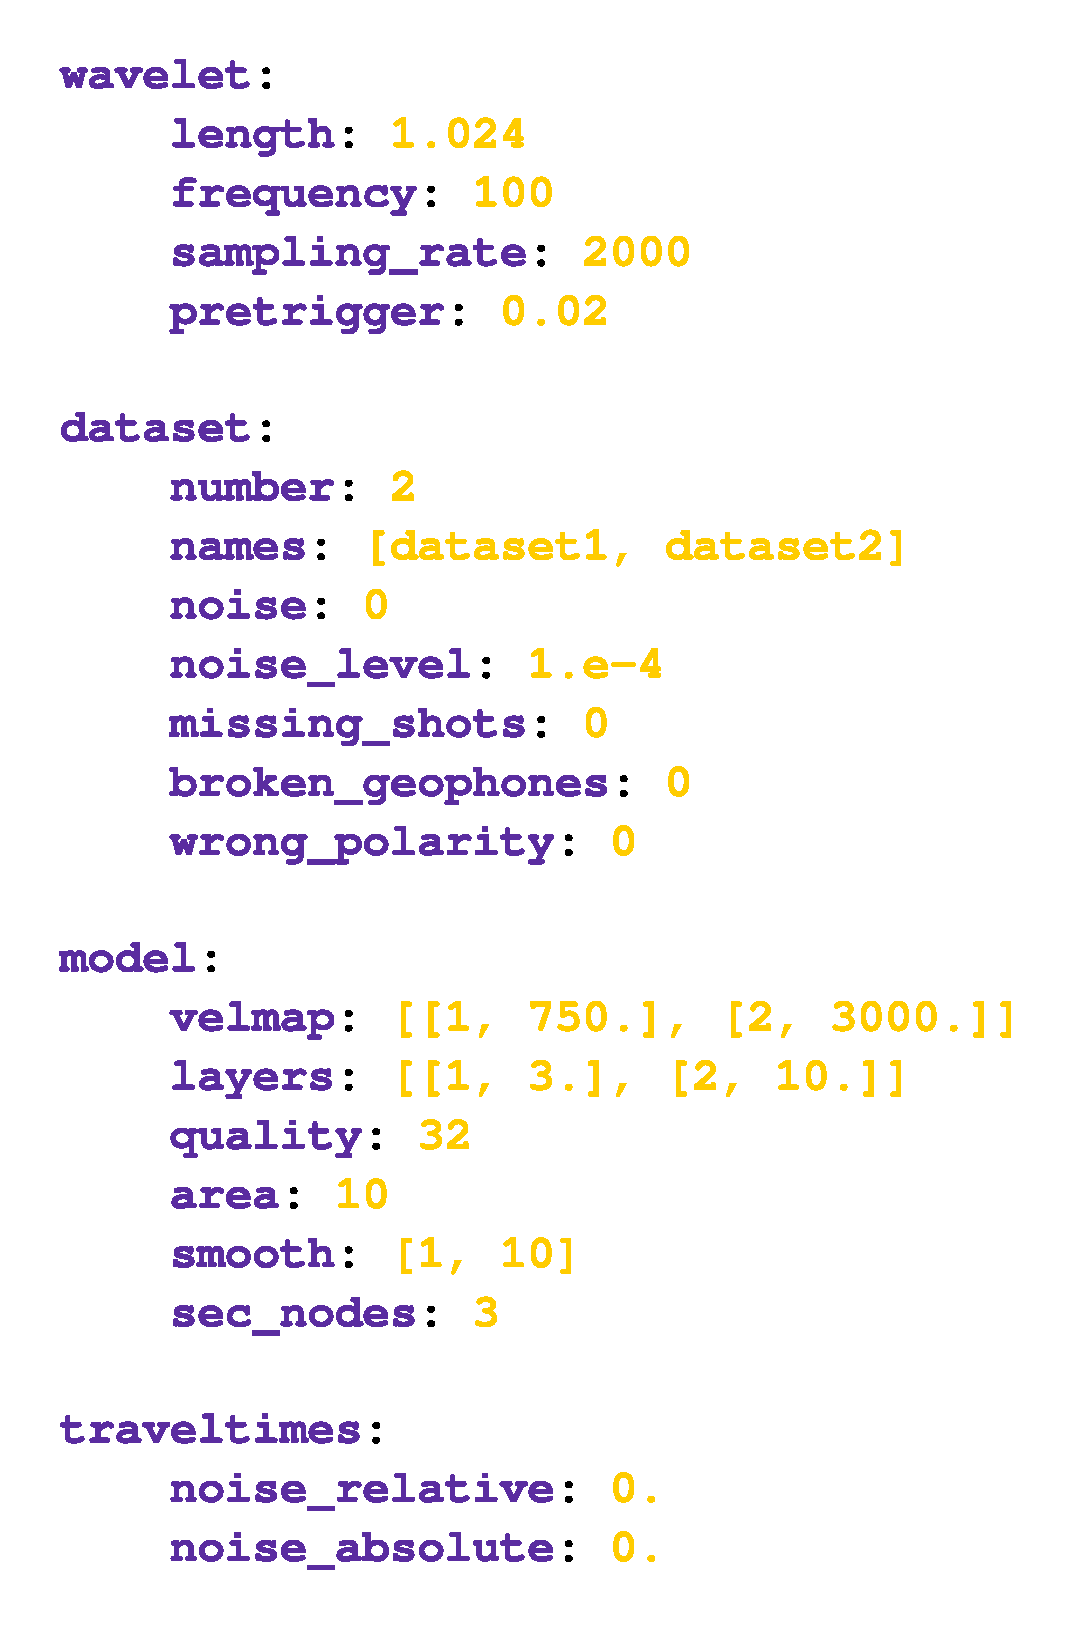
\includegraphics[width=.3\textwidth]{./figures/yaml_file.pdf}
\newline
In the exemplary configuration file shown above, the first block contains information regarding the wavelet, which controls the modeling of the seismic waveforms as described in Table~\ref{tab:config}.
In the second block, we can set specific names for the datasets to be created and the number of datasets is automatically determined. Alternatively, it is possible to set the number of datasets to be created and the dataset names are automatically generated with the prefix \textit{dataset\_}.
Various parameters control the random error (\texttt{noise}) and systematic errors in the modeled seismic waveform data (see Table~\ref{tab:config}).
The number and position of the shot and geophone stations affected by the systematic errors are randomly chosen with a maximum of 5\% of the total number of stations in order to avoid a high number of invalid trace data.
The third block contains information regarding the synthetic subsurface model. For each layer the corresponding velocity (\texttt{velmap}) and layer thickness (\texttt{layers}) need to be provided and all layers are considered to be parallel to the surface topography (geometrical information regarding the stations in the measurement scheme). The remaining parameters, namely \texttt{quality}, \texttt{area}, \texttt{smooth} and \texttt{sec\_nodes}, define the properties of the mesh to be used for the forward modeling (we refer to the respective pyGIMLi resources\footnote{https://www.pygimli.org/pygimliapi/\_generated/pygimli.meshtools.html\#pygimli.meshtools.createMesh, last accessed \today} for further information).
Alternatively, the user can provide a more complex mesh in the binary mesh format (i.e., a bms file):
\newline
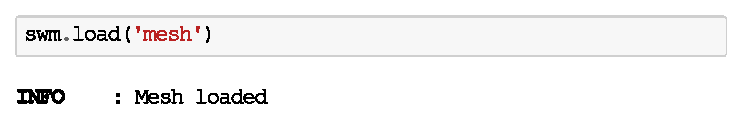
\includegraphics[width=.5\textwidth]{./figures/load_mesh.pdf}
\newline
The parameters in the final block control the forward modeling of the corresponding seismic traveltimes (see Table~\ref{tab:config}).
A configuration file located in the input directory can be imported through the \texttt{load} method:
\newline
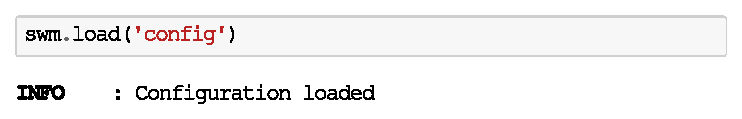
\includegraphics[width=.5\textwidth]{./figures/load_config.pdf}
\newline
\begin{table*}[]
    \caption{Description of the parameters, which can be defined in a configuration file used for the modeling of the synthetic seismic data.}
    \centering
    \begin{tabular*}{\tblwidth}{@{} LCL@{}}
        \toprule
        \textbf{Parameter} & \textbf{Unit/} & \textbf{Description} \\
         & \textbf{Data type} & \\ 
        \midrule
        \textbf{\texttt{wavelet}} & & \\
         & & \\
        length & s & Length of the base wavelet, which also defines the \\
         & & length of the synthetic seismic waveform data \\ 
        frequency & Hz & Frequency of the base wavelet \\ 
        sampling\_rate & Hz & Defines temporal resolution of the seismic waveforms \\ 
        pretrigger & s & Add buffer to the seismic waveforms before the onset \\
         & & of the actual data \\
        \midrule
        \textbf{\texttt{dataset}} & & \\
         & & \\
        number & int & Number of datasets to be created \\
        names & list (string) & Names of the datasets \\
        noise & bool & 1 in case noise should be added to the synthetic \\
         & & waveforms, 0 otherwise \\
        noise\_level & - & Level of the seismic background noise \\
        missing\_shots & bool & 1 in case the datasets should be affected by missing \\
         & & shot files, 0 otherwise \\
        broken\_geophones & bool & 1 in case the datasets should comprise broken \\
         & & geophones (i.e., no data in the corresponding \\
         & & seismograms), 0 otherwise \\
        wrong\_polarity & bool & 1 in case the datasets should contain traces with \\
         & & inverse polarity, 0 otherwise \\
        \midrule
        \textbf{\texttt{model}} & & \\
         & & \\
        velmap & list & For each layer the first value defines the marker and \\
         & (float/int) & the second one the seismic velocity within the layer \\
        layers & list & For each layer the first value defines the marker and \\
         & (float/int) & the second one the thickness \\
        \midrule
        \textbf{\texttt{traveltimes}} & & \\
         & & \\
        noise\_relative & \%/100 & Relative noise to be added to the forward modeled \\
      	 & & seismic traveltimes \\
        noise\_absolute & s & Absolute noise to be added to the forward modeled \\
         & & seismic traveltimes\\
        \bottomrule
    \end{tabular*}
    \label{tab:config}
\end{table*}
Once the \texttt{SeismicWaveformModeler} instance is parameterized the synthetic seismic waveform data can be created as follows:
\newline
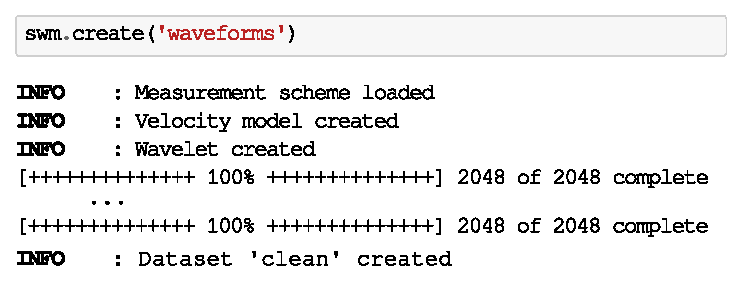
\includegraphics[width=.5\textwidth]{./figures/create_syn_data.pdf}
\newline
The \texttt{SeismicWaveformModeler} loads the measurement scheme 
and creates the velocity model used for the waveform modeling.
Based on the wavelet properties a Ricker wavelet is generated through the pyGIMLi function \texttt{ricker}.
Subsequently, mesh, velocity model and Ricker wavelet are used to solve the pressure wave equation for each shot station defined in the measurement scheme with the pyGIMLi function \texttt{solvePressureWave}.
The resultant waveforms at the corresponding geophone stations are extracted and stored in an ObsPy \texttt{Stream} data structure.
\clearpage
A directory for each dataset defined in the configuration file will be created in the output directory (\textit{out}):

\dirtree{%
.1 working\_directory.
.2 in.
.2 out.
.3 dataset1.
.4 data.
.5 protocol.txt.
.5 station\_coords.csv.
.5 Shot\_1001.syn.
.5 ....
.5 Shot\_10nn.syn.
.4 dataset1\_tt.pck.
.4 info.txt.
}
In the subdirectory \textit{data}, the synthetic seismic waveforms are stored in a separate shot file for each shot position in the miniseed format \citep{ahern2012, ringler2015} with the file extension \textit{syn} to identify the forward modeled shot files, e.g., Shot\_1001.syn.
The measurement protocol (protocol.txt) and the station coordinates provided as a csv file (station\_coords.csv) are also stored in this directory. The header of the measurement protocol contains the survey parameters required for the processing of the seismic waveforms, namely sampling rate, recording length, number of geophones and geophone spacing. Moreover, the protocol associates each shot file of the dataset to a specific location within the survey geometry, i.e., with respect to the geophone positions:
\newline
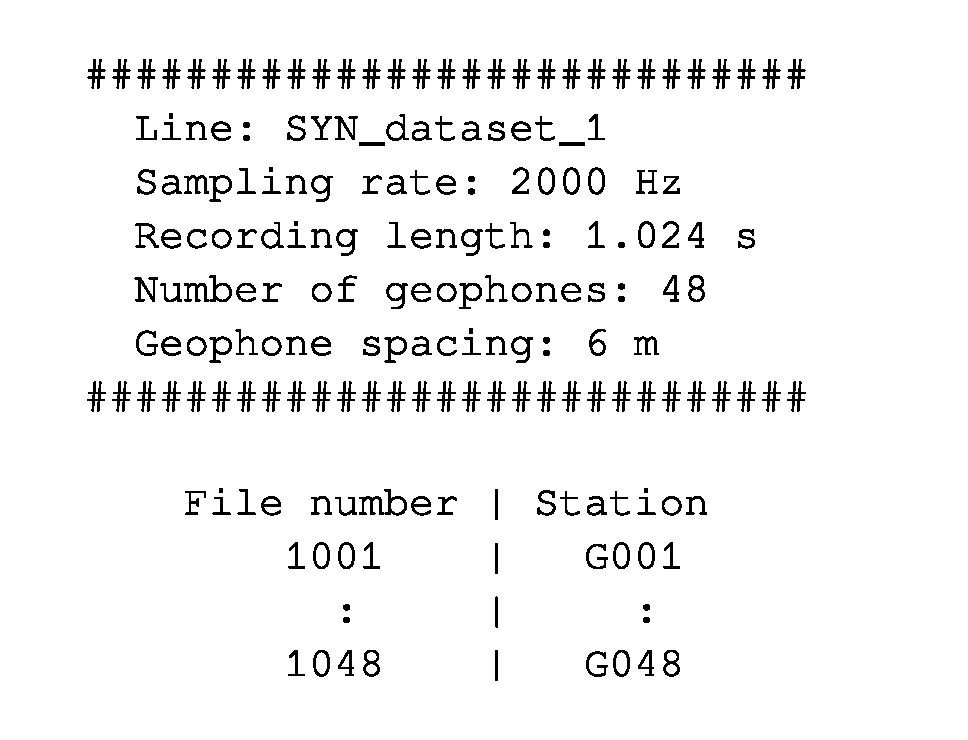
\includegraphics[width=.3\textwidth]{./figures/protocol.pdf}
\newline
The auxiliary file info.txt provided in the dataset directory summarizes the parameters from the configuration file and information regarding the simulated systematic errors in the synthetic seismic waveform data:
\newline
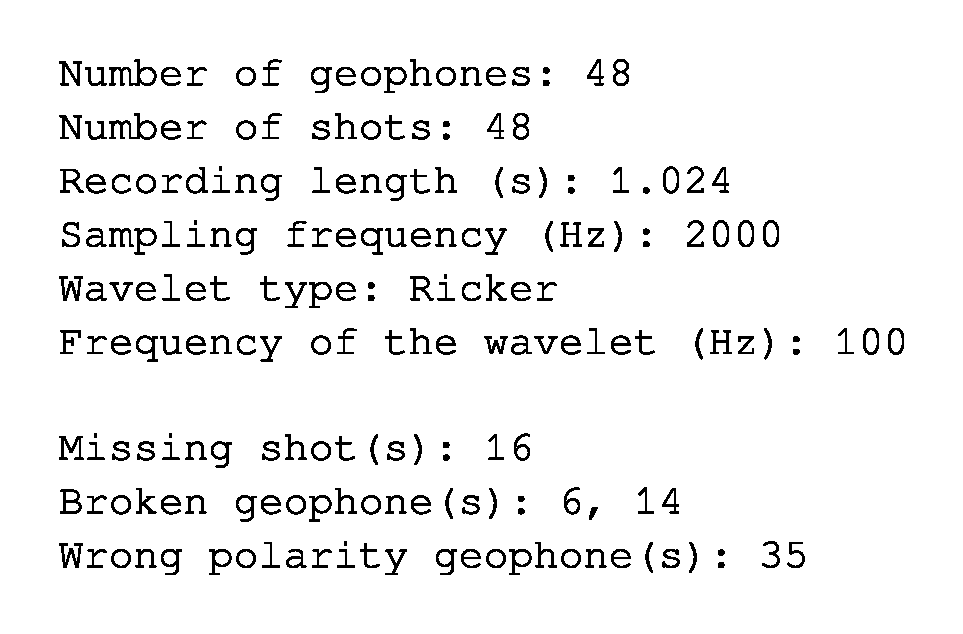
\includegraphics[width=.3\textwidth]{./figures/info.pdf}
\newline
Synthetic traveltimes (\texttt{swm.create('traveltimes')}) are stored in the dataset directory as udf files, e.g., dataset1\_tt.pck. The file extension \textit{pck} is an abbreviation of the word 'pick' and refers to the first break traveltimes saved in the file.

\subsection{Processing of seismic refraction datasets: the \texttt{SeismicRefractionManager}}

The SR method is based on the measurement of the traveltimes of seismic waves determined from the the first onset of the seismic energy recorded by geophones. In the SRT, the inversion of traveltimes gathered from tens to hundreds of seismograms permits the computation of variations in the seismic velocities in an imaging framework. Measuring the traveltimes in seismograms (i.e., first break picking) is commonly done manually (or semi-automatically) in an iterative process. The signal-to-noise ratio in the recorded seismograms substantially influences the quality of the traveltimes picked in the seismograms, and thus a proper enhancement of the perceptibility of the first onsets is crucial.

Accordingly, the \texttt{SeismicRefractionManager} class provides functionalities that permit the processing of seismic waveform data for a refraction seismic analysis. These functionalities involve the reading of seismic waveform data, combining the data with information about the survey geometry, processing of the waveforms as well as the picking of first break traveltimes. Since the first break picking is a highly interactive process, the \texttt{SeismicRefractionManager} is designed primarily for usage from within an ipython shell.

\subsubsection{Compiling the survey information and creating a project}

An instance of the \texttt{SeismicRefractionManager} can be created by providing the path to the working directory as parameter to the constructor. Based on the content of the working directory, the \texttt{SeismicRefractionManager} automatically decides whether (i) to start in the data preview mode, (ii) create a new project, or (iii) load an existing project from disk.

The data preview mode is primarily initiated if the provided working directory contains seismic shot files:
\newline
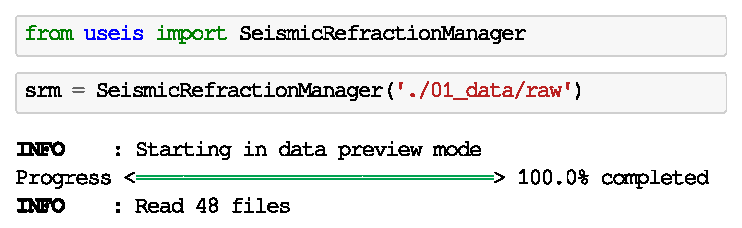
\includegraphics[width=.5\textwidth]{./figures/data_preview_mode.pdf}
\newline
To create or load a project, the working directory needs to contain specific subdirectories:

\dirtree{%
.1 working\_directory.
.2 01\_data.
.3 raw.
.2 02\_geom.
.2 03\_proc.
}
In this directory structure, the seismic shot files are stored in \textit{01\_data/raw} and the geometry file (\textit{geometry.csv}) is provided in \textit{02\_geom}.

The geometry file is a csv file that provides an abstract representation of the survey layout and must not contain a header. The fundamental element for the description of the survey layout is the station, which refers either to a geophone position, a shot position or a position with co-located shot and geophone. For each station the geometric and semantic information described in Table~\ref{tab:geometry} are provided column-wise, i.e., each line in the geometry file corresponds to a single station with a unique position within the survey layout. 
\begin{table}[pos=h]
    \caption{Description of the information to be provided in the columns of the geometry file.}
    \centering
    \begin{tabular}{clcl}
        \toprule
        Col & \textbf{Content} & \textbf{Data type} & \textbf{Description} \\
        \midrule
        1 & x coordinate & float & Station x coordinate, e.g., given in (m) \\ 
        2 & y coordinate & float & Station y coordinate, e.g., given in (m) \\ 
        3 & z coordinate & float & Station z coordinate, e.g., given in (m) \\ 
        4 & Geophone & bool & 1 if a geophone was deployed at station, 0 otherwise \\ 
        5 & Shot & int & The numerical part of the file name, e.g., 1001, if a shot was conducted \\
          & & & at this station, -1 otherwise \\ 
        6 & First geophone & int & First active geophone (-1 if no shot was conducted at the station) \\ 
        7 & Number of geophones & int & Number of active geophones (-1 if no shot was conducted at the station) \\
        \bottomrule
    \end{tabular}
    \label{tab:geometry}
\end{table}

In case the shot files as well as the geometry file are provided and a basic sanity check of the geometry file was successful, the \texttt{SeismicRefractionManager} creates a new project:
\newline
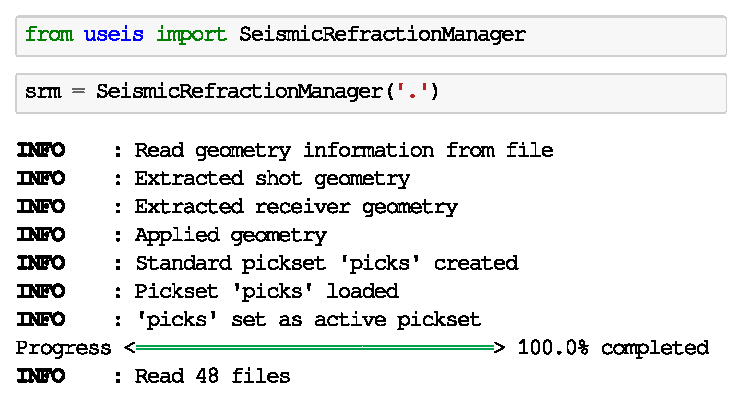
\includegraphics[width=.5\textwidth]{./figures/create_project.pdf}
\newline
In particular, the \texttt{SeismicRefractionManager} creates an SQLite database (prj.db in the working directory) to store the geometry information, whereby the stations are consecutively numbered (see Figure~\ref{fig:statnum}). To allow for an efficient data selection through the user the \texttt{SeismicRefractionManager} links the station numbers to shot index numbers (SIN) and receiver index numbers (RIN) assigned to shot and receiver stations, respectively (see Figure~\ref{fig:statnum}). Based on this information, the geometry is applied, i.e., the database tables required for the processing of the seismic waveform data are created.
In particular, the first break traveltimes for each SIN-RIN pair are stored in a dedicated database table \textit{fbpicks} together with the name of the corresponding pickset, i.e., the a common label for an entire set of first break traveltimes. By default, each project contains the default pickset 'picks', which is loaded and activated on startup. Once the database is initialized, the waveform data are read from disk and the project is ready for processing.
\begin{figure}
	\centering
	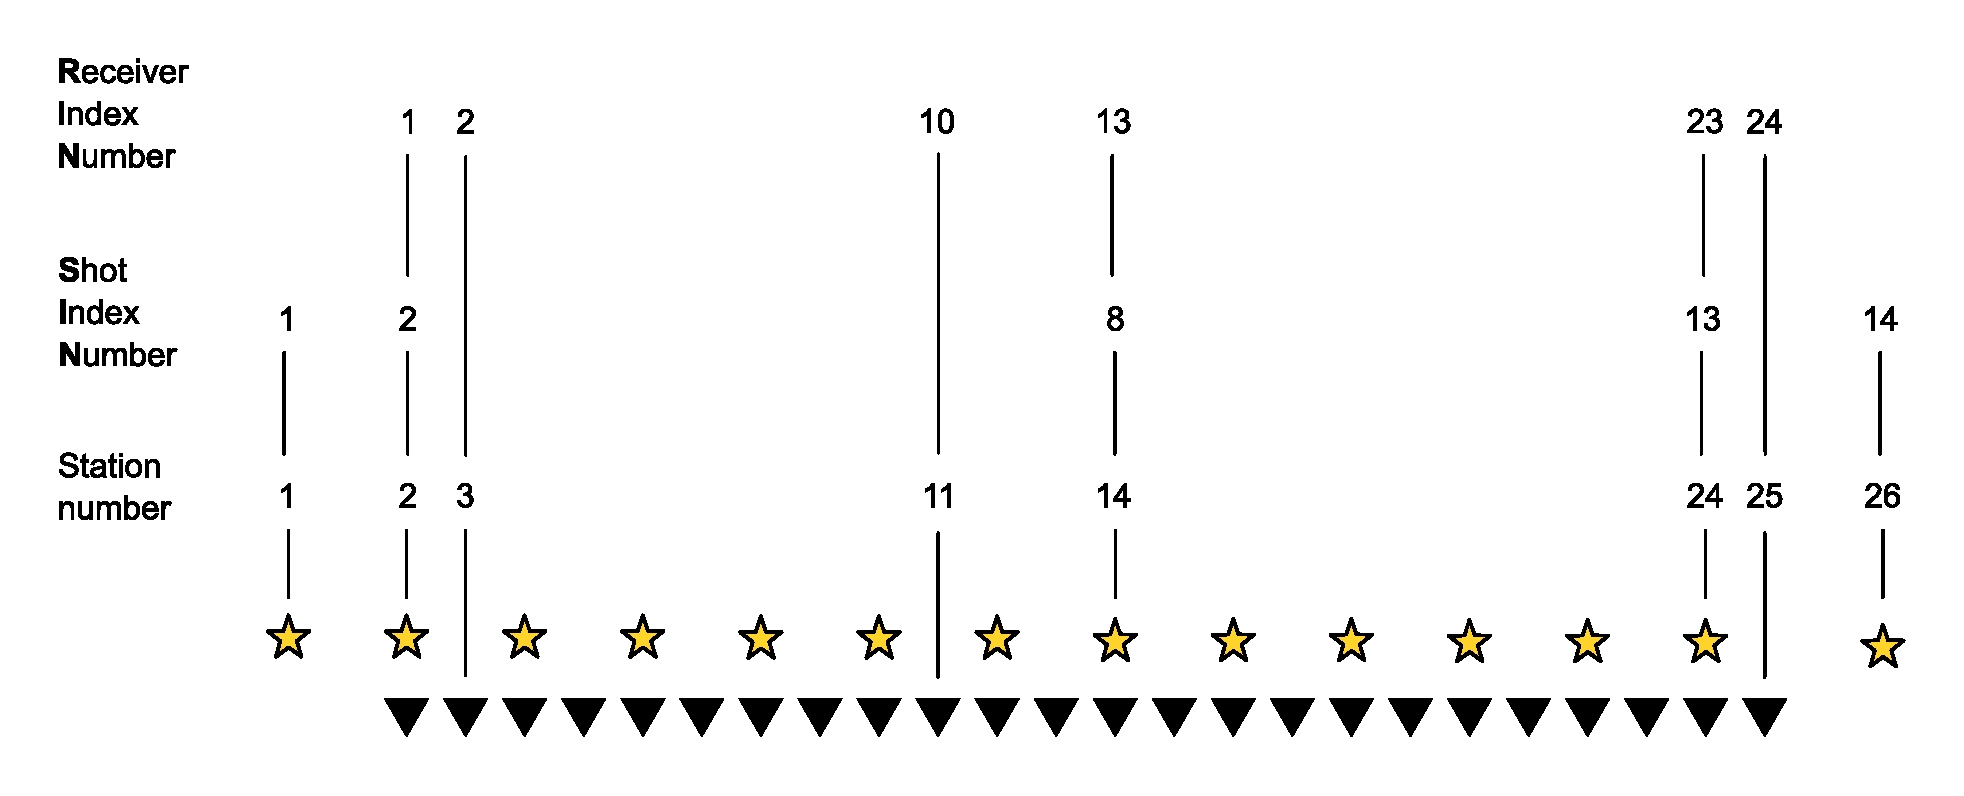
\includegraphics[width=.75\textwidth]{figures/station_numbering.pdf}
	\caption{The \texttt{SeismicRefractionManager} addresses the stations through consecutive station numbers based on the sort order in the geometry file. The shot index numbers (SIN) and receiver index numbers (RIN) are assigned to the shot and receiver stations separately to allow for an intuitive data handling for the user.}
	\label{fig:statnum}
\end{figure}

If a database file is already present in the working directory, the project information, the seismic waveforms as well as the default pickset 'picks' are automatically loaded:
\newline
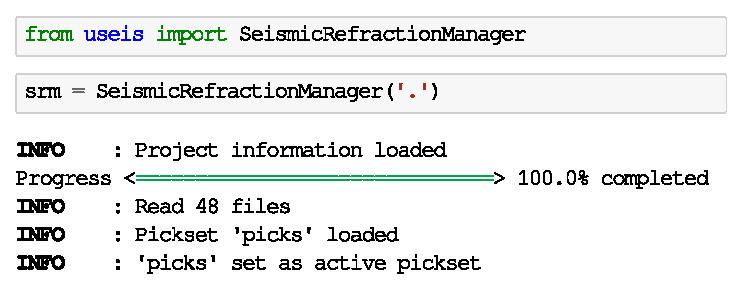
\includegraphics[width=.5\textwidth]{./figures/load_project.pdf}

For a project with a successfully applied geometry, the \texttt{select} method of the \texttt{SeismicRefractionManager} allows to gather the seismic waveforms based on a common shot (\texttt{sin}), a common receiver (\texttt{rin}) or the common absolute offset (\texttt{aoffset}):
\newline
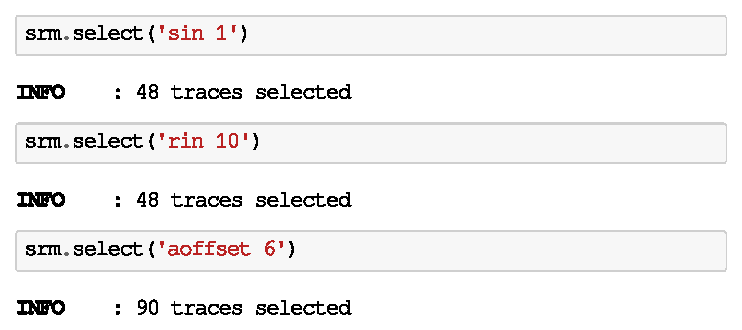
\includegraphics[width=.5\textwidth]{./figures/select.pdf}

\subsubsection{Visualization and enhancement of the seismic waveform data}
Calling the \texttt{plot} method without passing any parameter allows for the visualization of the currently selected traces:
\newline
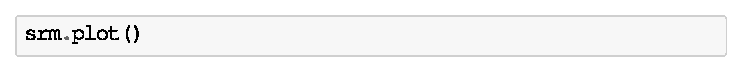
\includegraphics[width=.5\textwidth]{./figures/plot.pdf}
\newline
Once opened, the seismogram plot visualizes the seismic waveforms in a combination of wiggle trace and variable area mode, i.e., the trace data are shown as curves. The area of the curves is colored red for negative and blue for positive amplitudes, respectively (not shown for brevity). Pressing the up or down arrow key on the keyboard toggles the visualization mode between variable area and variable density. In variable density mode the strength of the amplitudes is additionally reflected by the color saturation, i.e., high amplitudes refer to a stronger shade than low amplitudes (see Figure~\ref{fig:srm_intro}).
\begin{figure}
	\centering
	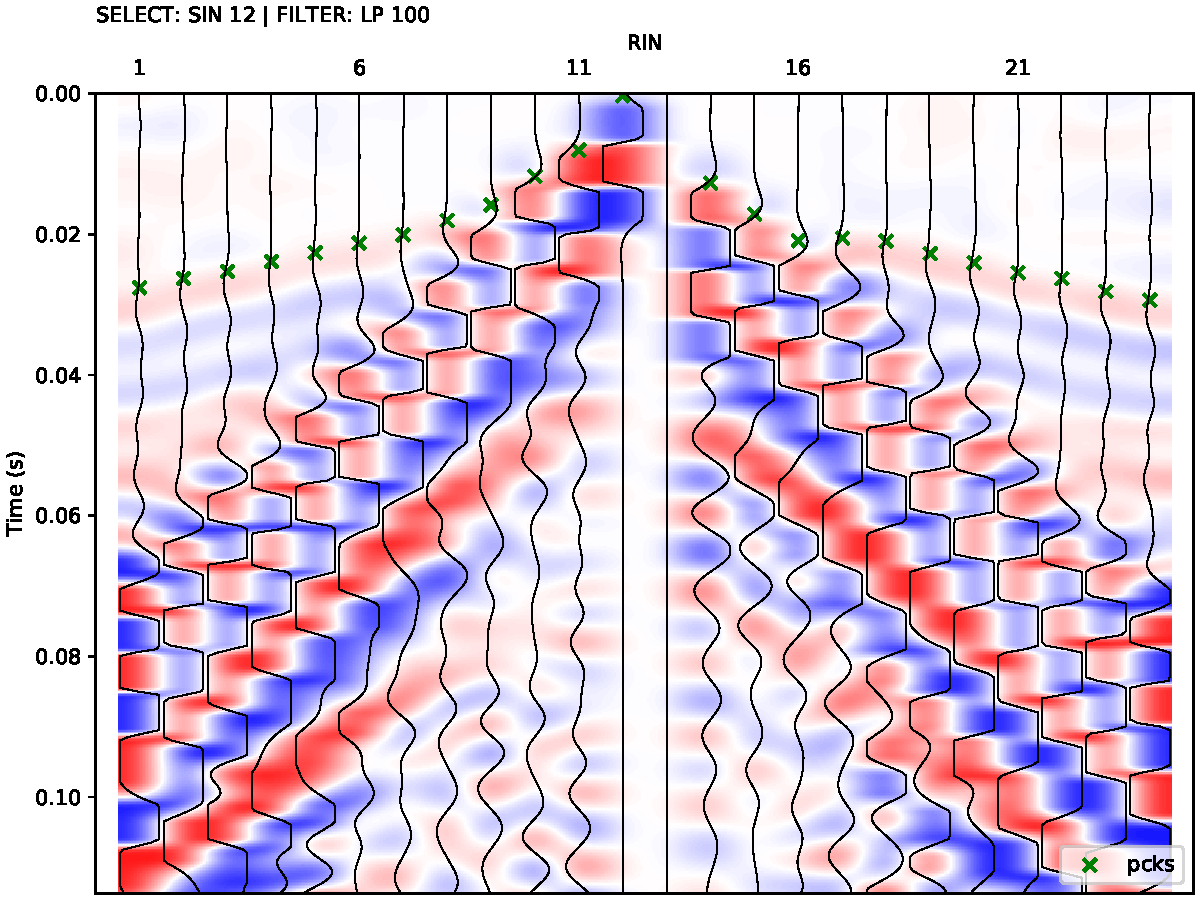
\includegraphics[width=.75\textwidth]{figures/pickwindow_intro.pdf}
	\caption{The seismogram plot presents the currently selected traces along the x axis, where the sort order is determined through the geometry. The corresponding trace data are illustrated as a function of time along the y axis (solid curves), with positive and negative amplitudes depicted in blue and red, respectively. The selection criterion and the applied filter are shown in the upper left corner of the plot. Green crosses refer to the picked traveltimes stored in the currently active pickset.}
	\label{fig:srm_intro}
\end{figure}

The active processing mode and data scaling mode are reported together with the traveltime at the current cursor position in the status bar of the seismogram plot window (see Figure~\ref{fig:statusbar_intro}).
The initial processing mode is 'Fb pick', i.e., first break picking is possible. The user can switch between the different modes by pressing specific keys on the keyboard. The 'm' key activates the trace mute mode ('Trc mute'), which allows to set the amplitude of a trace to zero by clicking with the left mouse button; clicking again on the same trace restores the amplitude information. The trace reverse mode ('Trc rev') is activated by pressing the 'r' key and enables the user to toggle the polarity of a trace by clicking on it with the left mouse button. 
The default data scaling mode is 'Zoom', which allows the scaling of the y-axis by turning the mouse wheel. By pressing the 'a' key the amplitude scaling mode ('Amp scal') is activated. Turning the mouse wheel increases or decreases the amplitudes of the traces currently shown in the seismogram plot, and thus might help to enhance the perceptibility of the first onsets.
By pressing the key of the currently active mode again, the \texttt{SeismicRefractionManager} returns to the default mode; yet, the different modes can be activated in any arbitrary order (as illustrated in Figure~\ref{fig:statusbar_intro}).
\begin{figure}
	\centering
	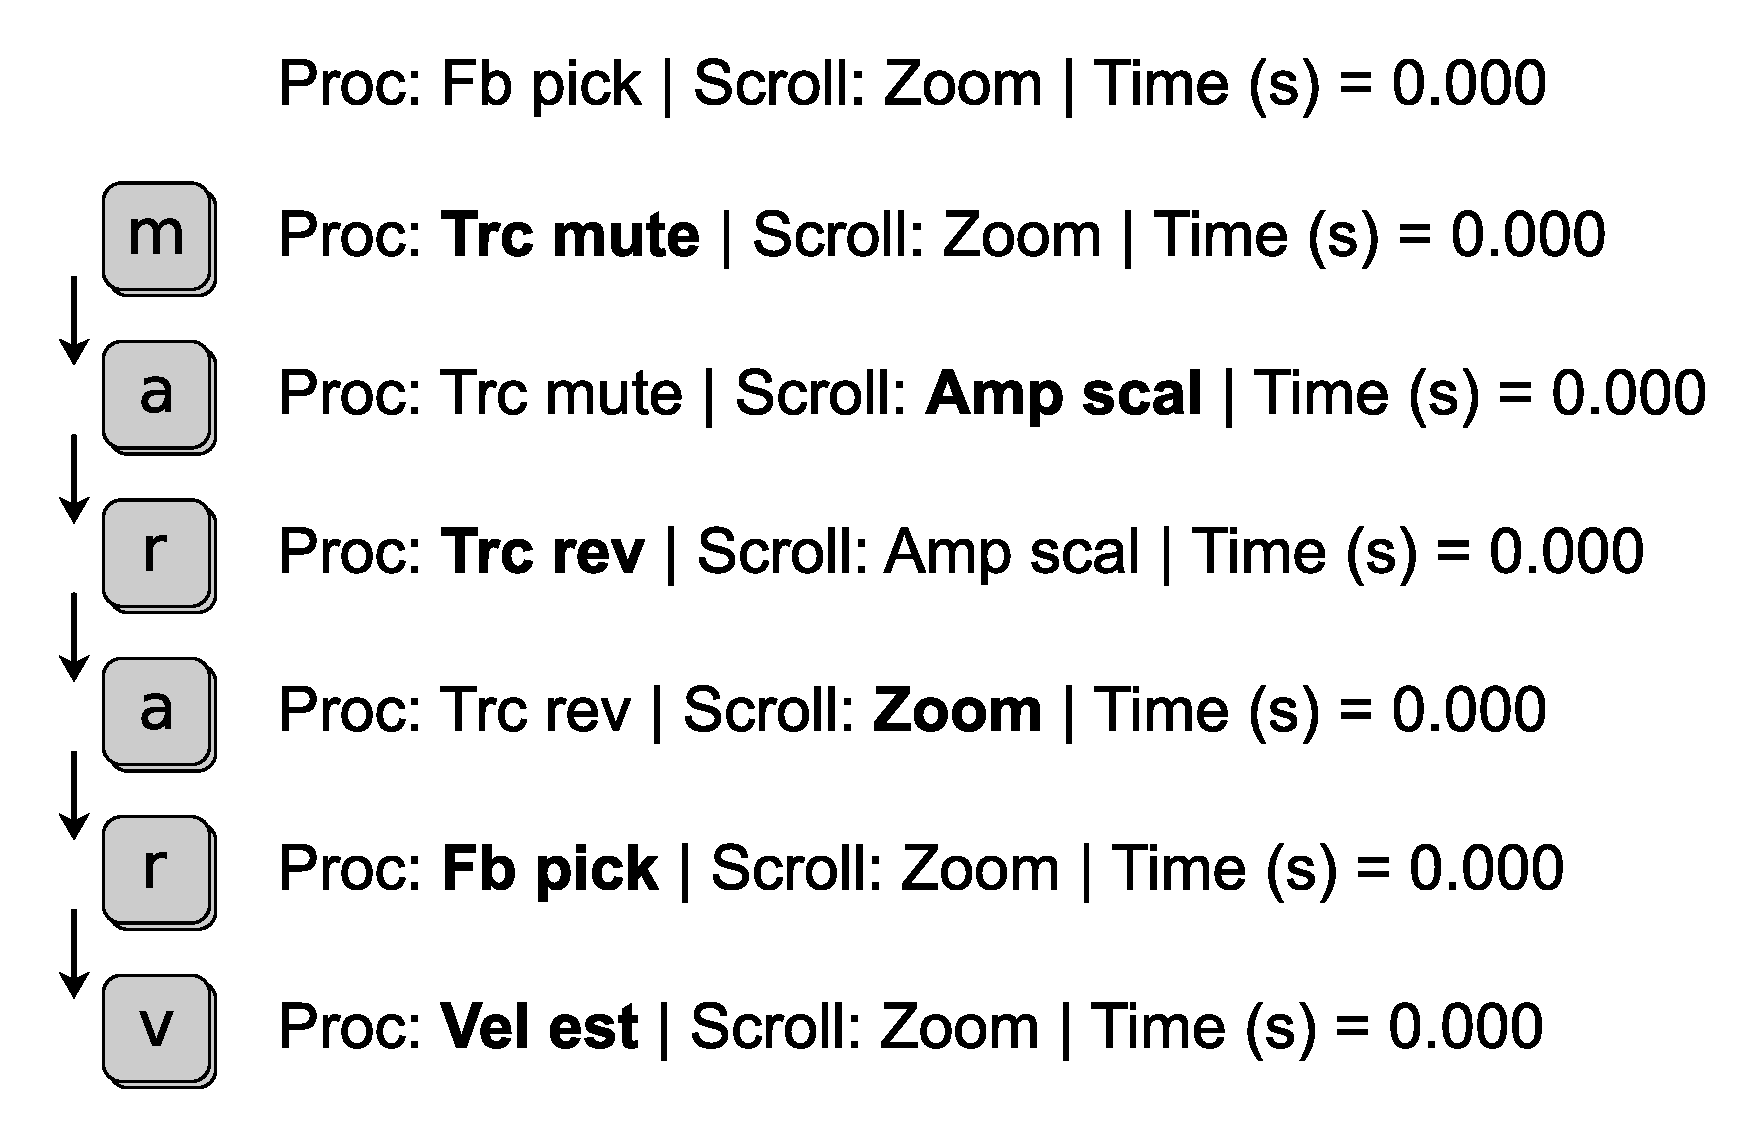
\includegraphics[width=.75\textwidth]{figures/status_bar.pdf}
	\caption{The status bar in the interactive seismogram plot displays the currently active processing and data scaling modes as well as the time (in seconds) at the current cursor position. By pressing the keys 'a', 'm', 'r', 'v' on the keyboard the different modes can be activated.}
	\label{fig:statusbar_intro}
\end{figure}

Through the \texttt{plot} method the frequency spectrum of the currently selected trace data can be visualized:
\newline
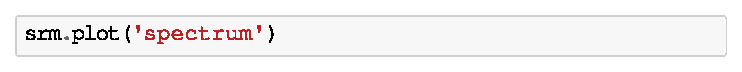
\includegraphics[width=.5\textwidth]{./figures/plot_spectrum.pdf}
\newline
A frequency spectrum as shown in Figure~\ref{fig:spectrum} can be used to discriminate the dominating signal frequencies from those associated to the background noise, and thus allows for the definition of adequate filter settings.
\begin{figure}
	\centering
	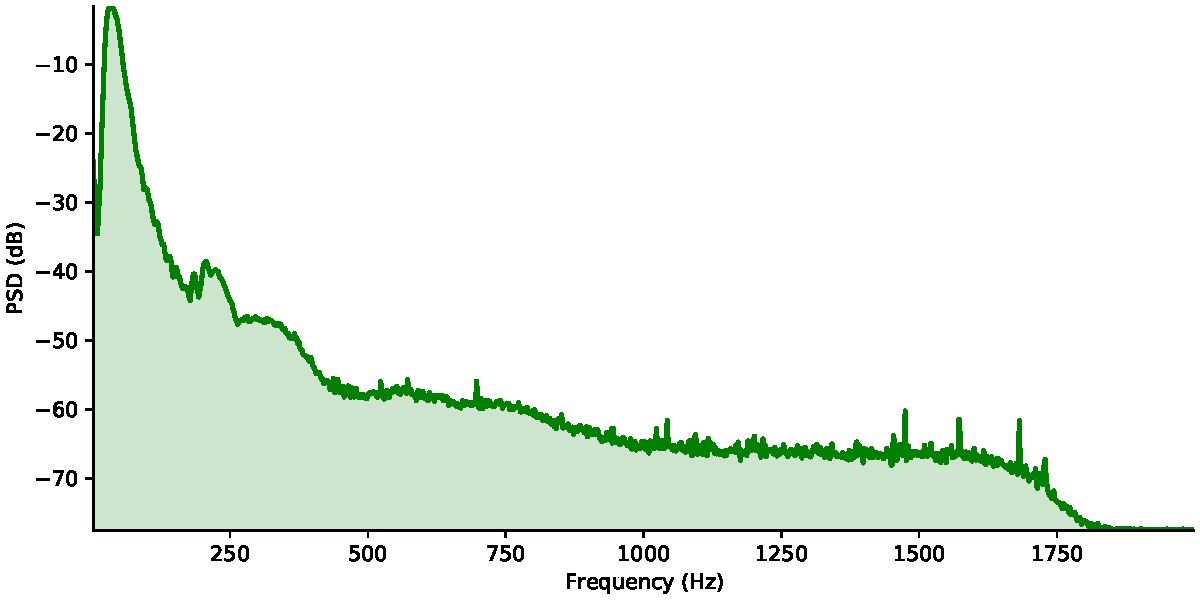
\includegraphics[width=.75\textwidth]{figures/spectrum.pdf}
	\caption{The frequency spectrum illustrates the frequency content of the currently selected traces, which allows for the identification of frequency ranges associated to noise, which can be omitted through the application of corresponding frequency filtering.}
	\label{fig:spectrum}
\end{figure}
To improve the signal-to-noise ratio it is possible to apply filters on the selected traces through the \texttt{filter} method, which utilizes the frequency filters implemented in the ObsPy package \citep[lowpass, highpass, bandpass and bandstop;][]{beyreuther2010}, e.g.:
\newline
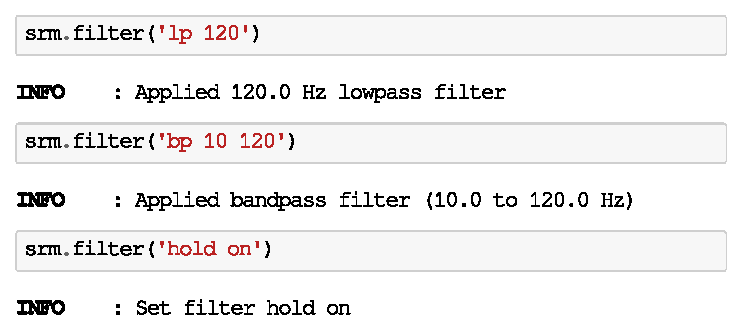
\includegraphics[width=.5\textwidth]{./figures/filter.pdf}
\newline
By default, filters are solely applied to the currently selected traces, yet setting the filter on hold allows the filtering of all subsequently selected traces with the same filter settings.
In case the seismogram plot is opened, the effect of the applied filter on the seismic waveforms is interactively visualized.

\subsubsection{Analysis of the seismic waveforms and first break traveltime picking}

In the seismogram plot, the waveforms can be analyzed and processed to obtain information about the subsurface conditions. Activating the velocity estimation mode ('Vel est') by pressing the 'v' key on the keyboard, enables the user to estimate velocities for different wave phases (e.g., originating from a refractor) by pressing the left mouse button and moving the cursor. Once the left mouse button is released, a line between the start and end point is drawn and labeled with the corresponding velocity (estimates can be deleted by clicking with the right mouse button).

If the processing mode 'Fb pick' is activated, picking of first break traveltimes is done individually by clicking with the left mouse button on the respective trace. Clicking again on the same trace will set the first break pick to the new location as there can only be one traveltime for each SIN-RIN pair; whereas clicking with the right mouse button deletes the pick. Alternatively, first break picks can be set for multiple traces by pressing the left mouse button and moving the cursor. 
Once the left mouse button is released, first break picks are defined at the intersections between the line and the seismograms. In the same way, multiple picks can be deleted if a line is drawn with the right mouse button pressed. The first break traveltimes determined in the seismogram plot are automatically written to the project database when the window is closed or another set of traces is loaded by pressing the 'left' or 'right' arrow keys on the keyboard. 

The traveltime diagram for the currently active pickset can be created through the \texttt{plot} method:
\newline
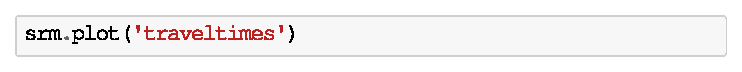
\includegraphics[width=.5\textwidth]{./figures/plot_traveltimes.pdf}
\newline
Figure~\ref{fig:traveltimes_intro} presents an exemplary traveltime diagram, which is a common way to examine the quality of the first break picking. Such illustration of the traveltimes can be used to identify outliers or erroneous measurements, which are commonly associated to traveltimes with substantial deviations from those observed at adjacent stations such as the first break pick for the SIN-RIN pair (23, 11). Outliers can be removed by clicking on the corresponding symbol ('x') in the traveltime diagram, which is instantly synchronized with the project database. If the seismogram plot and the traveltime diagram are used side-by-side, changes made to the first break picks in one window will interactively trigger an update of the other one and vice versa.

\begin{figure}
	\centering
	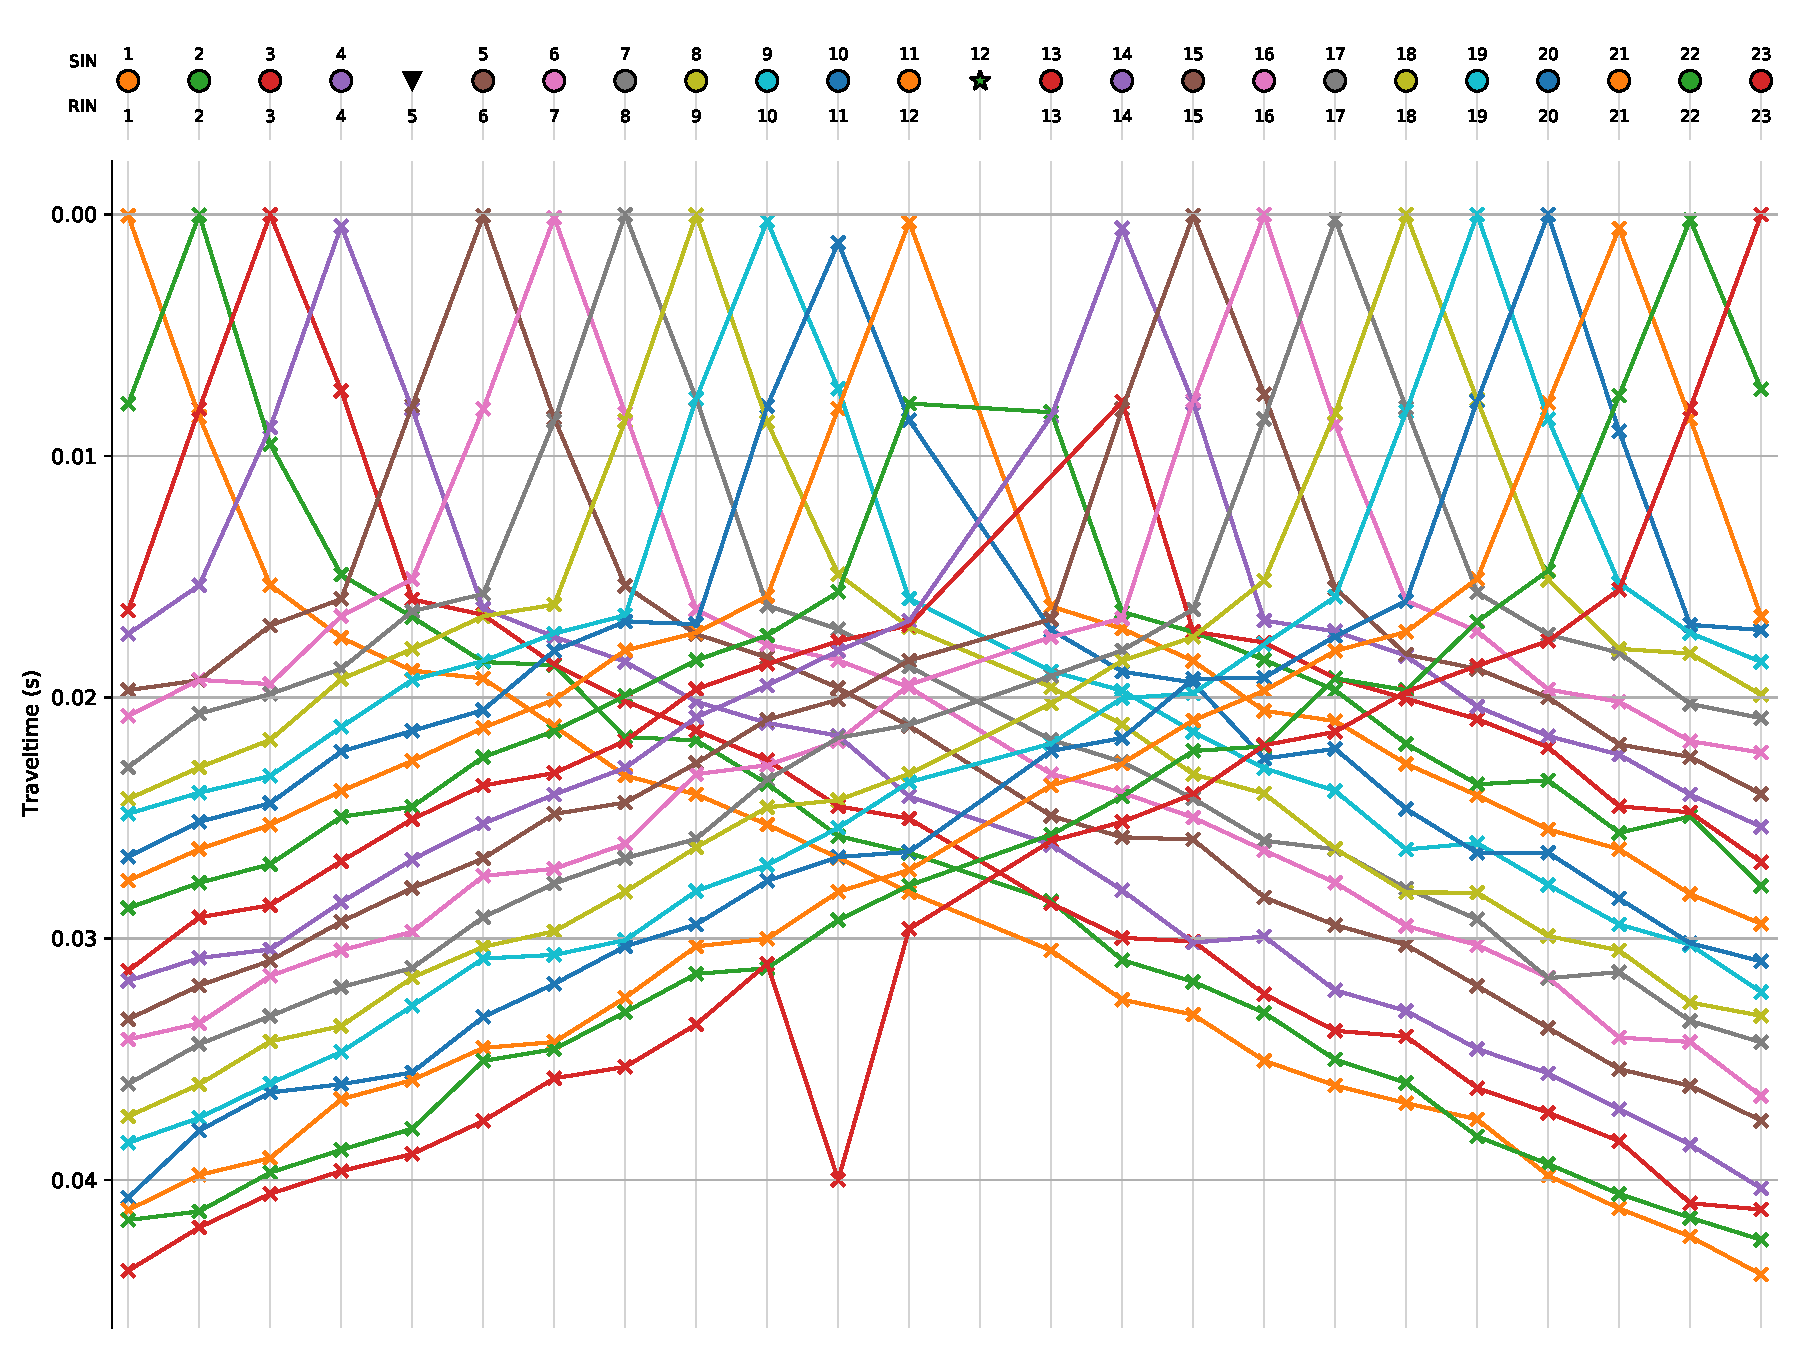
\includegraphics[width=.75\textwidth]{figures/traveltimes_intro.pdf}
	\caption{The traveltime diagram shows the first break traveltimes stored in the currently active pickset along the y axis (x symbols), where solid lines connect traveltimes assigned to a common shot. The sort order of the stations along the x axis reflects the geometry. Filled circles indicate stations with co-located shot and geophone (receiver), triangles refer to receiver stations (no shot) and stars refer to shot stations (no geophone).}
	\label{fig:traveltimes_intro}
\end{figure}

The \texttt{SeismicRefractionManager} handles first break picks in picksets, which can be organized and manipulated through the \texttt{picksets} method of the \texttt{SeismicRefractionManager}:
\newline
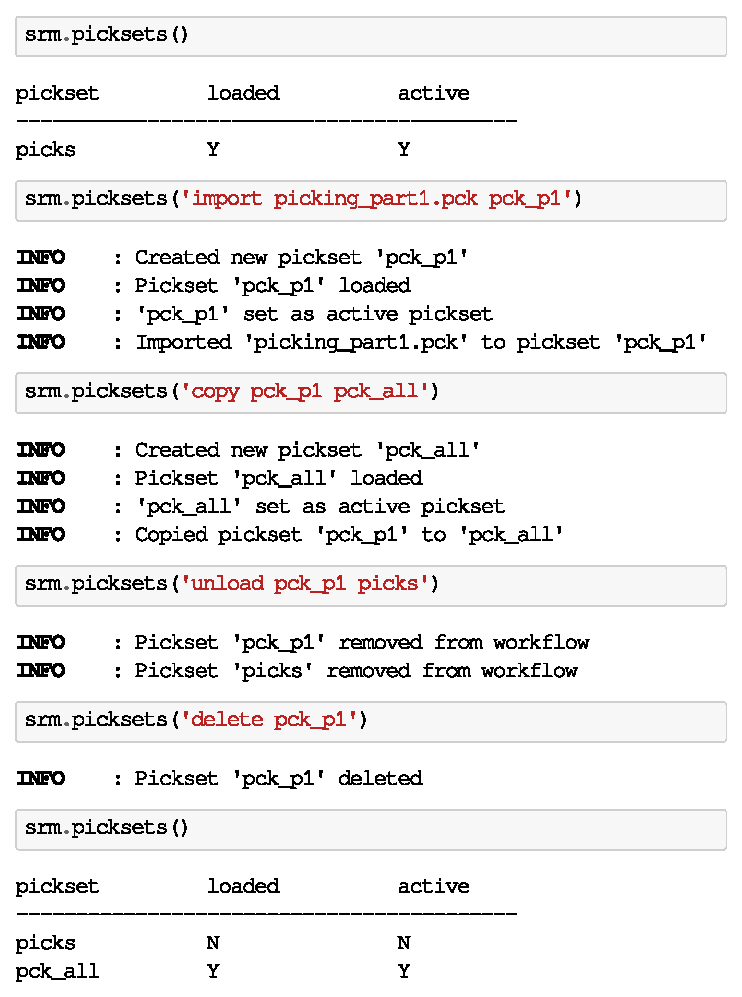
\includegraphics[width=.5\textwidth]{./figures/picksets.pdf}
\newline
Calling the \texttt{pickset} method without parameters shows the status of all picksets in the project. From the above use case, we see that by default, the pickset 'picks' is loaded and activated, i.e., modifications of first breaks are stored in this pickset. First break picks provided by another source (as udf file) can be imported from  \textit{03\_proc/picks}.
For the first break picking, it is sufficient to keep only one pickset in the workflow, i.e., not required picksets can be unloaded. A pickset currently not loaded can be deleted permanently, i.e., the corresponding traveltimes are removed from the database. The \texttt{picksets} method can also be used to load picksets from the database:
\newline
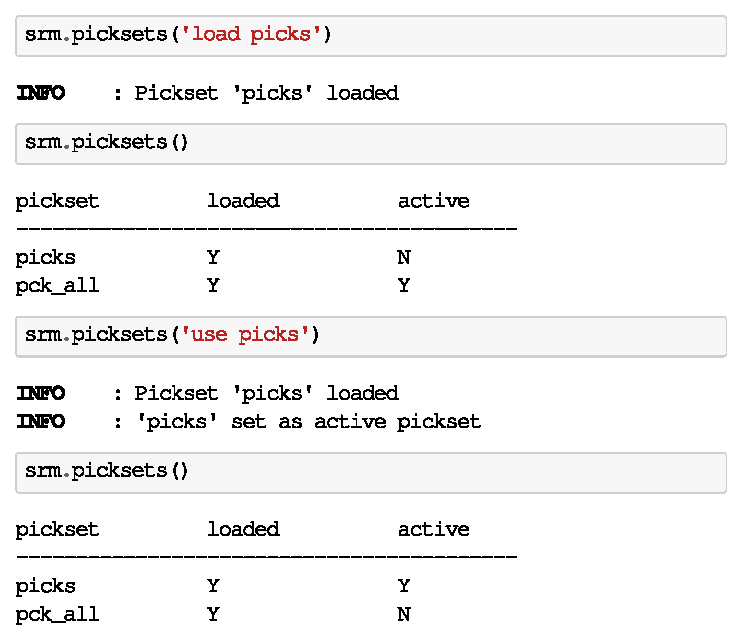
\includegraphics[width=.5\textwidth]{./figures/load_picksets.pdf}
\newline
When a pickset is loaded from the database, it does not become the active pickset automatically; whereas by using the parameter \texttt{use} the corresponding pickset is loaded and also becomes the active pickset. The first break traveltimes of a pickset can be exported to an udf file that is stored in \textit{03\_proc/picks} subdirectory with the current timestamp as suffix:
\newline
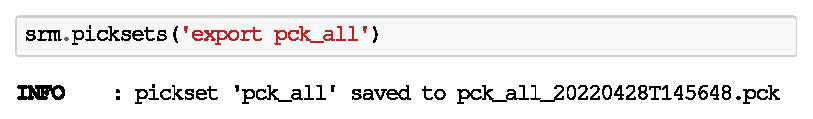
\includegraphics[width=.5\textwidth]{./figures/export_pickset.pdf}

\section{Exemplary use cases}

\subsection{Modeling and use of synthetic seismic waveform data}

To demonstrate the applicability of the \texttt{SeismicWaveformModeler} class, we generate two synthetic seismic waveform datasets assuming two horizontal layers in a half-space without topography and an interface between these layers with a constant depth.
Table~\ref{tab:syndata} summarizes the parameterization used for the forward modeling of one dataset without noise (Dataset\_1) and another dataset containing random noise and systematic errors (Dataset\_2).
For the visualization of both synthetic datasets, we provide the corresponding geometry files to the \texttt{SeismicRefractionManager} in order to have full control regarding data selection and processing capabilities. 

The synthetic seismic waveforms for SIN 24 of Dataset\_1 presented in Figure~\ref{fig:syndata_clean} reveal clear negative first onsets 
%in all traces.
%From these seismograms, we can also identify 
and allow the identification of crossover points, i.e., inflexion points between the first arrivals from the first layer (RIN 17 to 30) and the first onsets associated to the second layer (RIN 1 to 16 and RIN 31 to 48). 
%In Figure~\ref{fig:syndata_noise}, we present the synthetic seismic waveforms from Dataset\_2 for the same shot (SIN 24). 
In contrast 
%to Dataset\_1, 
the signal-to-noise ratio of Dataset\_2 (see Figure~\ref{fig:syndata_noise}) is a function of the offset between shot and geophone position, i.e., traces farther away from the shot contain a higher level of random noise. 
Moreover, Dataset\_2 also contains systematic errors, where RIN 6 and 14 refer to broken geophones, and RIN 35 is an example for readings with a wrong polarity.
We believe that such synthetic datasets might be useful for investigating the effect of complex survey geometries on seismic data as well as the development and evaluation of processing strategies.
\begin{table}[pos=h]
    \caption{Measurement scheme and parameters provided in the yaml files used to create synthetic seismic waveform datasets with (Dataset\_1) and without added noise (Dataset\_2).}
    \centering
    \begin{tabular}{lcc}
        \toprule
        \textbf{Measurement scheme} & & \\
        Number of stations & 48 & \\
        Station spacing & 2\,m & \\
        Number of geophones & 48 & \\
        Number of shots & 48 & \\
        \midrule
        \textbf{Model} & \textit{Layer 1} & \textit{Layer 2} \\
		Thickness & 3\,m & 10\,m \\
        Velocity & 750\,m/s & 3000\,m/s \\
        \midrule
        \textbf{Dataset} & \textit{Dataset\_1} & \textit{Dataset\_2} \\
		Noise & False & True \\
		Noise level & 0 & 1e-5 \\
		Missing shots & False & True \\
		Broken geophones & False & True \\
		Wrong polarity & False & True \\
		\midrule
		\textbf{Wavelet} & & \\
		Length & 1.024\,s & \\
		Frequency & 100\,Hz & \\
		Sampling rate & 2000\,Hz & \\
        \bottomrule
    \end{tabular}
    \label{tab:syndata}
\end{table}
\begin{figure}
	\centering
	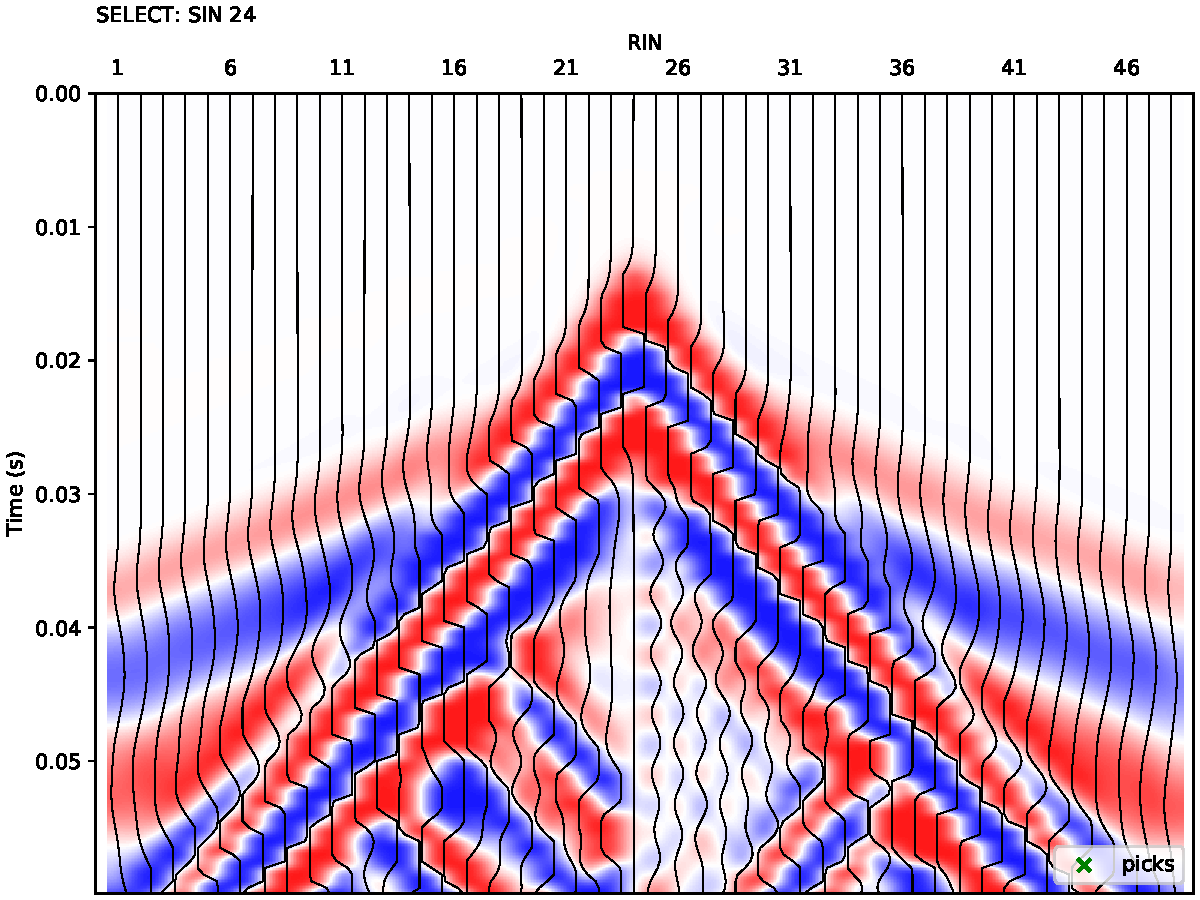
\includegraphics[width=.75\textwidth]{figures/syn_clean_sin24.pdf}
	\caption{Synthetic seismic waveform data without random or systematic errors created with the \texttt{SeismicWaveformModeler()} class for a shot position in the center of the survey layout.}
	\label{fig:syndata_clean}
\end{figure}

\begin{figure}
	\centering
	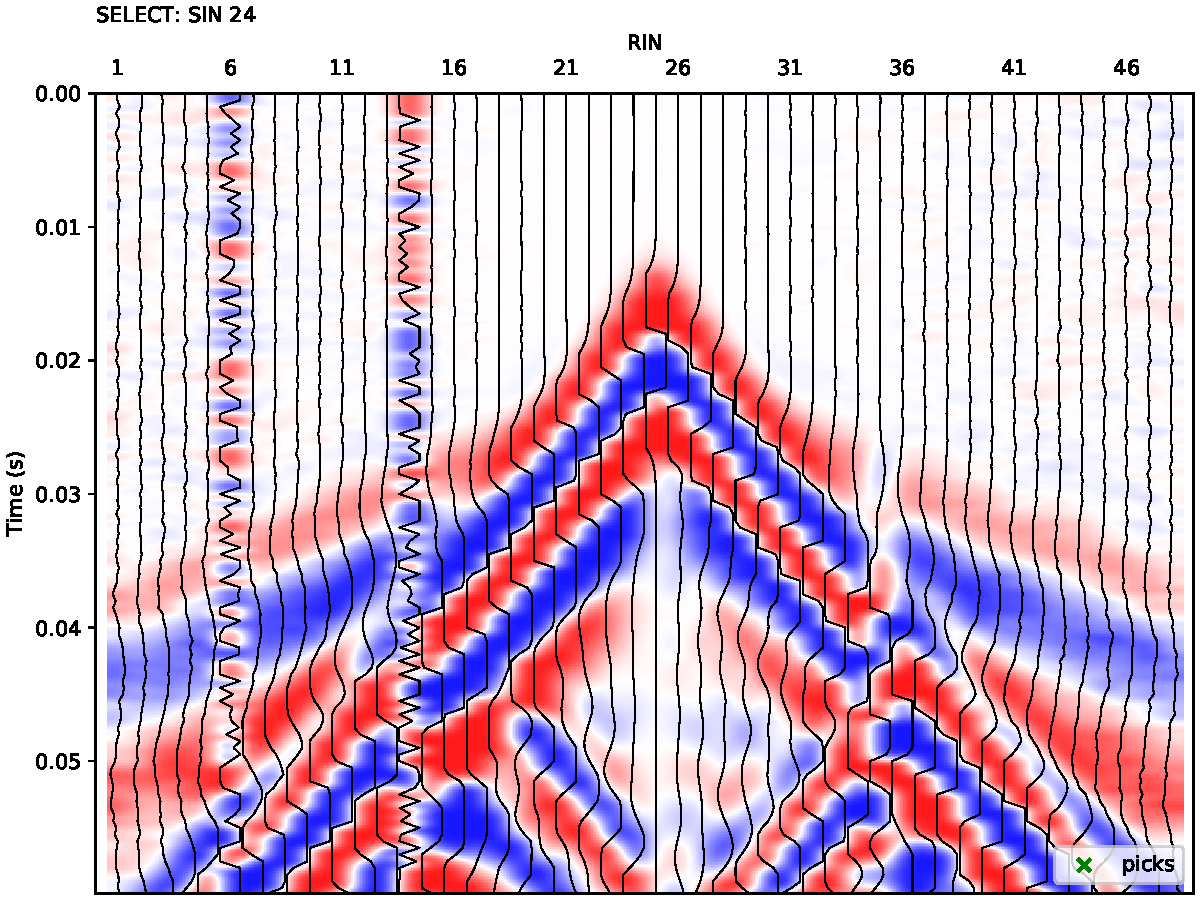
\includegraphics[width=.75\textwidth]{figures/syn_noise_sin24.pdf}
	\caption{Synthetic seismic waveform data with added noise created with the \texttt{SeismicWaveformModeler()} class for a shot position in the center of the survey layout. The random noise refers to an offset dependent decrease of the signal-to-noise ratio, while the systematic broken geophones and wrong polarity are systematic errors.}
	\label{fig:syndata_noise}
\end{figure}

Accordingly, the concept of the formikoj library 
%and the \texttt{SeismicRefractionManager} 
allows the implementation of supplementary functionalities. 
Such custom extensions should be implemented either as internal methods or as functions in the utilities module, which are then executed through the \texttt{compute} method with a custom keyword. 
%We illustrate this possibility for customization through the implementation of
As an illustrative example, we implemented 
a simplified version of an automatic first break picking algorithm, which determines the traveltimes based on the energy ratio method \citep[e.g.,][]{earle1994}. The algorithm is added to the \texttt{SeismicRefractionManager} in form of two internal methods \texttt{\_manage\_autopicking} and \texttt{\_compute\_autopicks}, respectively. The autopicking process can be started by passing the new keyword \texttt{autopick} as the first parameter to the \texttt{compute} method:
\newline
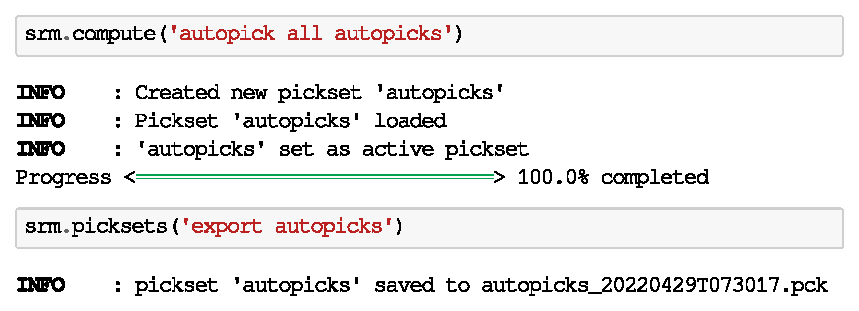
\includegraphics[width=.5\textwidth]{./figures/autopicking.pdf}
\newline
The second parameter defines whether traveltimes should be determined for 
%automatic first break picking should be applied to 
the entire dataset (\texttt{all}) or solely for the currently selected traces (\texttt{cur}). The third parameter provides the name of the corresponding pickset in the % for the automatically determined first break traveltimes. 
%Accordingly, the traveltimes are stored in the 
project database; thus, making the traveltimes available for visualization and processing with existing functionalities or further custom implementations.

\subsection{First break travel time picking for a 2D roll-along field data set: the Danube island example}

The seismic data used in this example were collected at the Danube island (Vienna) in June 2021, using 48 geophones deployed with 2\,m spacing between them and shot locations located between the geophone positions. As illustrated in Figure~\ref{fig:map_danube}, the survey geometry refers to a roll-along geometry, i.e., the geophone spread was moved along a profile with 50\% overlap yielding a total of five segments. The objective of the survey was to define the contact between different sediments within the tertiary and quarternary deposits used to build the man-made Danube island. Additionally, the survey aimed to identify lateral changes that might indicate the position of a fault, which has been inferred from sediments recovered from drillings. 
\begin{figure}
	\centering
	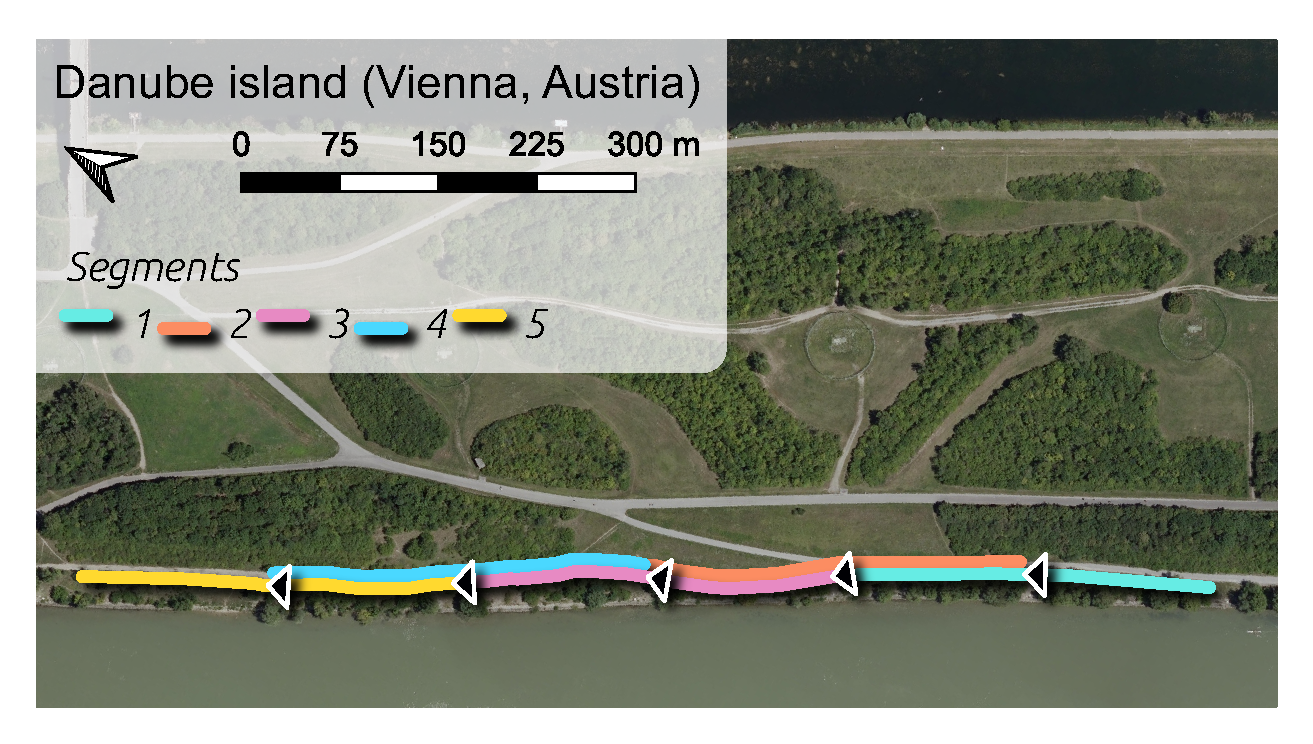
\includegraphics[width=.75\textwidth]{./figures/map_danube.pdf}
	\caption{The Danube island field dataset was collected along a single line with a roll-along survey layout; the filled triangles indicate the direction of the measurements. The five segments have an overlap of 50\% to ensure an adequate data coverage along the entire profile.}
	\label{fig:map_danube}
\end{figure}

\begin{table}[pos=h]
   \caption{Extract from the roll-along survey geometry file showing how the information regarding the first geophone assigns the traces in the shot files to the correct stations.}
    \centering
    \begin{tabular}{rrrcrrr}
        \toprule
        \textbf{x (m)} & \textbf{y (m)} & \textbf{z (m)} & \textbf{Geo} & \textbf{Shot} & \textbf{1st Geo} & \textbf{\# Geo} \\
        \midrule
        0.0 & 0.0 & 163.5 & 1 & -1 & -1 & -1 \\
        2.0 & 0.0 & 163.5 & 0 & 1001 & \textbf{1} & 48 \\
        \vdots & \vdots & \vdots & \vdots & \vdots & \vdots & \vdots \\
        94.0 & 0 & 163.5 & 0 & 1024 & \textbf{1} & 48 \\
		96.0 & 0 & 163.5 & 1 & -1 & -1 & -1 \\
        98.0 & 0.0 & 163.5 & 0 & 1037 & \textbf{25} & 48 \\
        \vdots & \vdots & \vdots & \vdots & \vdots & \vdots & \vdots \\
		194.0 & 0.0 & 163.5 & 0 & 1049 & \textbf{25} & 48 \\		
		196.0 & 0.0 & 163.5 & 1 & -1 & -1 & -1 \\        
        198.0 & 0.0 & 163.5 & 0 & 1073 & \textbf{49} & 48 \\
        200.0 & 0.0 & 163.5 & 1 & -1 & -1 & -1 \\
        202.0 & 0.0 & 163.5 & 0 & 1050 & \textbf{25} & 48 \\
        \vdots & \vdots & \vdots & \vdots & \vdots & \vdots & \vdots \\
        286.0 & 0.0 & 163.5 & 0 & 1084 & \textbf{49} & 48 \\
        288.0 & 0.0 & 163.5 & 1 & -1 & -1 & -1 \\
        290.0 & 0.0 & 163.5 & 0 & 1097 & \textbf{73} & 48 \\
        \vdots & \vdots & \vdots & \vdots & \vdots & \vdots & \vdots \\
		386.0 & 0.0 & 163.5 & 0 & 1109 & \textbf{73} & 48 \\
        388.0 & 0.0 & 163.5 & 1 & -1 & -1 & -1 \\
		390.0 & 0.0 & 163.5 & 0 & 2025 & \textbf{97} & 48 \\
		\vdots & \vdots & \vdots & \vdots & \vdots & \vdots & \vdots \\
		570.0 & 0.0 & 163.5 & 0 & 2048 & \textbf{97} & 48 \\		
		572.0 & 0.0 & 163.5 & 1 & -1 & -1 & -1 \\
        \bottomrule
    \end{tabular}
    \label{tab:rollalong_geometry}
\end{table}

In the field, each segment was measured separately, yet for the processing all measurements are combined in a single profile. %, i.e., the stations of all segments are consecutively numbered.
We can implement such measurement layout in a geometry file 
%of the \texttt{SeismicRefractionManager} 
as illustrated in Table~\ref{tab:rollalong_geometry}. %To describe a roll-along survey 
The key parameter is '1st Geo' as it indicates the first active geophone along the profile for each shot file. For the first segment in a roll-along survey geometry, the first active geophone is always geophone 1. Considering the number of geophones used in each segment, and an overlap of 50\%, the first geophone for segments two to five are 25, 49, 73 and 97, respectively.
%By providing these values in the geometry file as shown in Table~\ref{tab:rollalong_geometry}, the \texttt{SeismicRefractionManager} can apply the geometry information in the project database.

\begin{figure}
	\centering
	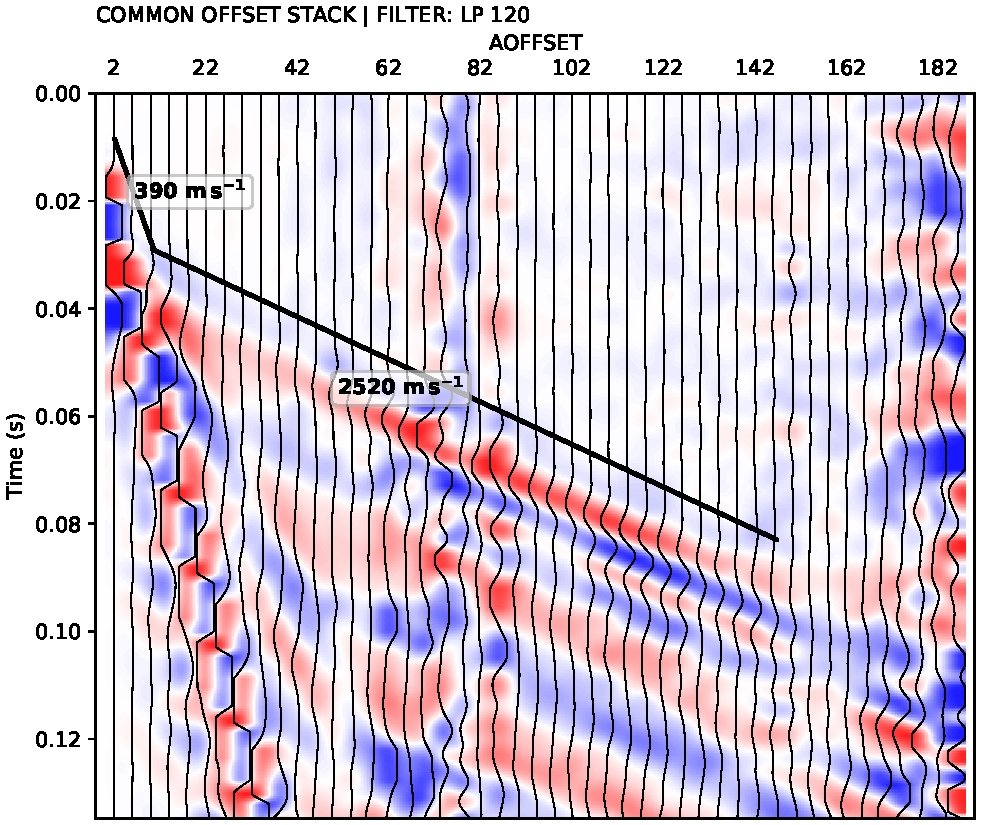
\includegraphics[width=.75\textwidth]{figures/danube_island_cos_lp120.pdf}
	\caption{The common offset stack computed for the Danube island dataset clearly showing a two-layered subsurface. The seismic velocities within the layer can be estimated from the gradient of the lines drawn along the corresponding first onsets of the seismic waves.}
	\label{fig:fieldcos}
\end{figure}

Based on the shot files and the geometry file stored in the required directory structure the \texttt{SeismicRefractionManager} creates the project database.
%Once the geometry is applied, i.e., the project is ready for processing, we can obtain 
A first illustration of the subsurface conditions can be obtained by computing a common offset stack (COS):
\newline
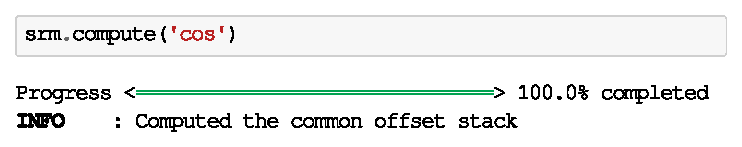
\includegraphics[width=.5\textwidth]{./figures/plotcos_danube.pdf}
\newline
%For the common offset stack, all traces with the same absolute offset from a shot point are stacked, i.e., compute the mean of the summed trace data. In this way, we can reduce the influence of the incoherent noise and thus improve the signal-to-noise ratio. 
The COS for the Danube island dataset presented in Figure~\ref{fig:fieldcos} shows first onsets for absolute offsets up to approximately 150\,m, which suggest a two-layered subsurface model. By using the velocity estimation functionality we can approximate the seismic velocity in the corresponding layers.

%After getting a first impression of the subsurface conditions, we can start 
For the first break picking a set of traces is selected, filtered if necessary and visualized:
\newline
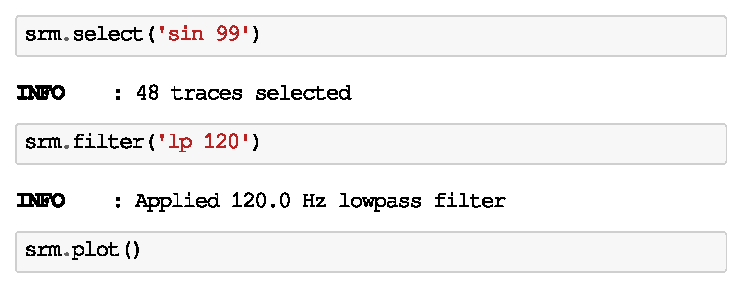
\includegraphics[width=.5\textwidth]{./figures/plotsin99_danube.pdf}
\newline
In this example, the trace data for SIN 99 are used, which refers to a shot position located in segment four. 
%We can easily verify this in the seismogram plot presented in Figure~\ref{fig:rollalong_pickwindow}, where the lowest RIN (along the x-axis) is 73, corresponding to the first active geophone defined for this segment.
As can be seen in Figure~\ref{fig:rollalong_pickwindow}, the first onsets are easily identifiable despite the substantial seismic background noise at large offsets (RIN 73 to 90).
\begin{figure}
	\centering
	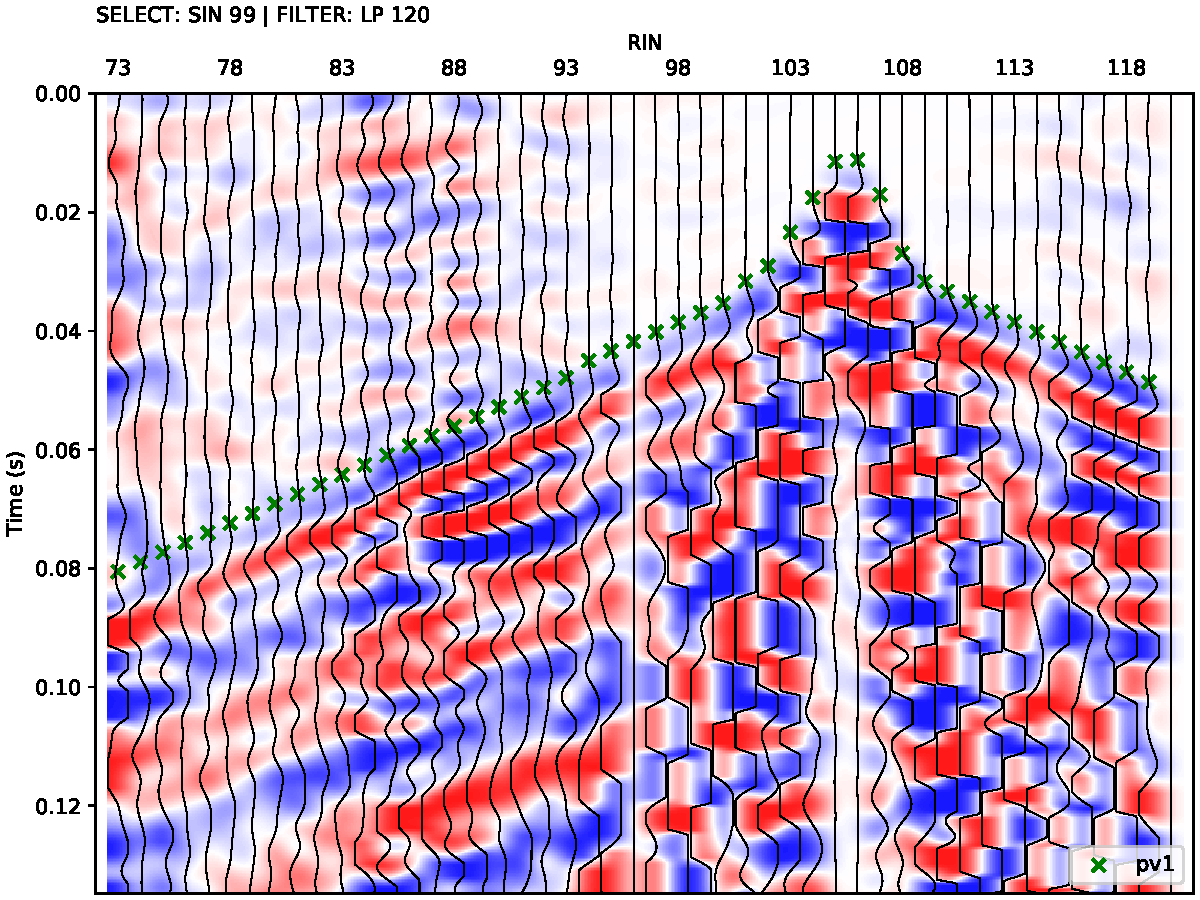
\includegraphics[width=.75\textwidth]{figures/danube_island_sin99_lp120_picks_vd.pdf}
	\caption{Examplary seismic waveforms from the Danube island dataset shown for shot index number (SIN) 99 with a 120 Hz lowpass filter applied to suppress high frequency noise. The receiver index numbers (RIN) start at 73, thus indicating that the data were collected with a roll-along survey geometry.}
	\label{fig:rollalong_pickwindow}
\end{figure}
A pseudosection provides an illustration of the corresponding apparent seismic velocity values computed from the picked traveltimes and the distance between shots and geophones:
\newline
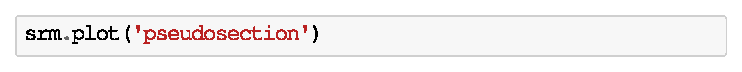
\includegraphics[width=.5\textwidth]{./figures/plotpseudosection_danube.pdf}
%\newline

%Such pseudosection can be created through the \texttt{plot} method of the \texttt{SeismicRefractionManager}:
In a pseudosection, as presented in Figure~\ref{fig:rollalong_pseudosection} for the Danube island dataset, the apparent velocity values are assigned to pseudolocations, with the corresponding x- and z-coordinates determined as the midpoint and as $1/3$ of the absolute offset between the shot and geophone, respectively.
Accordingly, such plot allows for the identification of outliers in the data, e.g., stark velocity contrasts for adjacent points, or systematic errors, e.g., velocities erroneously influenced by a single shot or receiver. The main assumption here is that the pseudosection should reveal smooth transitions between lateral and vertical neighbors, considering that the data were collected with gradual changes in the position of the source (i.e., hammer blow) and the receiver (i.e., geophone). The pseudosection will reveal large variations in case of abrupt changes in the topography or the geometry of the array, yet this can be taken into account by the user 
%during the evaluation of the pseudosection aiming at 
during the identification of outliers and possible systematic errors.
For the Danube island dataset, the pseudosection suggests an increase in the seismic velocity along profile direction in deeper subsurface regions (i.e., larger pseudodepth). Such pattern could be related to a fault expected in this area of the Danube island, thus indicating that the geophysical survey was sufficiently designed to detect such feature.
%conducted in an appropriate location to detect the fault.
Moreover, the pseudosection presented in Figure~\ref{fig:rollalong_pseudosection} shows a low number of data points in the first segment of the Danube island survey. This lack of data points at large pseudodepths is due to a low number of picked traveltimes at large offsets, and thus might indicate a low signal-noise ratio.
\begin{figure}
	\centering
	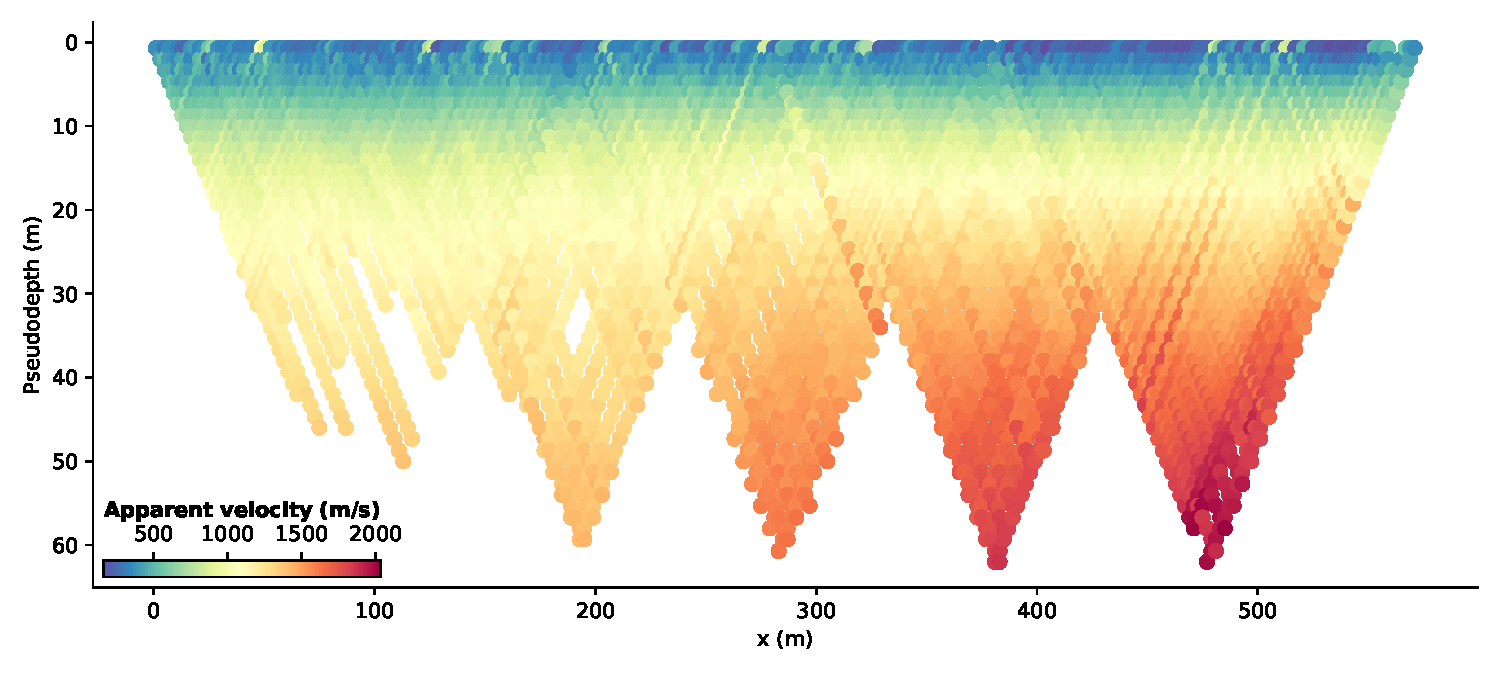
\includegraphics[width=.75\textwidth]{figures/rollalong_pseudosection.pdf}
	\caption{Pseudosection showing the apparent seismic velocities determined from the first break traveltimes obtained from the Danube island dataset and the corresponding absolute offset between the shot and receiver stations. The apparent velocity for each shot-receiver pair is illustrated at the corresponding midpoint and pseudodepth (1/3 of the absolute offset).}
	\label{fig:rollalong_pseudosection}
\end{figure}

%The \texttt{SeismicRefractionManager} also provides the possibility to 
To review the data quality along the entire profile it is possible to visualize the picking percentage, i.e., the ratio of actually picked traveltimes and total number of SIN-RIN pairs:
\newline
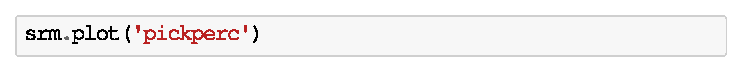
\includegraphics[width=.5\textwidth]{./figures/plot_pickperc_danube.pdf}
\newline
Figure~\ref{fig:rollalong_pickperc} shows that the picking percentage is visualized separately for each SIN. In this way, a low picking percentage indicates shots affected by a low signal-to-noise ratio. For the Danube island dataset, the picking percentage is low in the first segment, which confirms the lack of datapoints observed in the pseudosection. Moreover, the picking percentage plot can be used to track the picking progress, for instance 
%. In case of a large dataset, for which the 
if the traveltimes cannot be determined in one session or 
%, the picking percentage plot provides information where to resume the first break picking in the next session. Moreover, it is possible 
to identify single shots that might have been forgotten during the first break picking. Accordingly, it is advisable to check the picking percentage prior to exporting the traveltimes for the inversion.

\begin{figure}
	\centering
	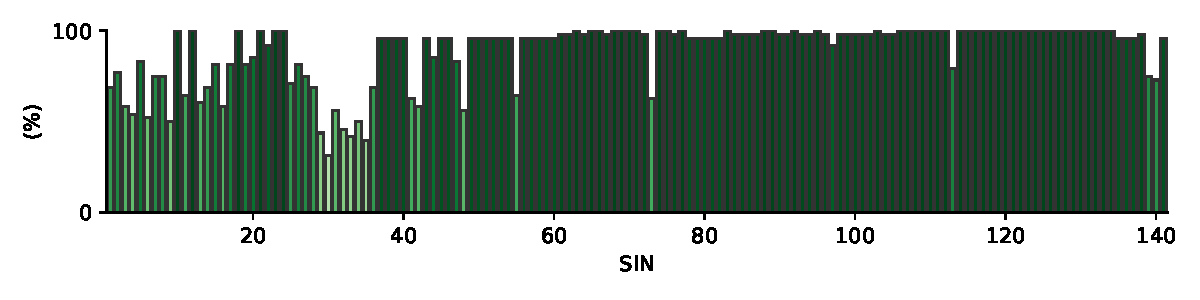
\includegraphics[width=.75\textwidth]{figures/rollalong_pickperc.pdf}
	\caption{Picking percentage for each shot in the Danube island roll-along dataset. Low values in the first third of the dataset indicate a low signal-to-noise ratio in the seismograms hindering the picking of first break traveltimes for each shot-receiver pair.}
	\label{fig:rollalong_pickperc}
\end{figure}
\subsection{Processing of a 3D seismic refraction dataset: the soda lake example}

The \texttt{SeismicRefractionManager} allows also the visualization and processing of data collected with a 3D survey layout. To illustrate these capabilities, we present in Figure~\ref{fig:map_sodalakes} the geometry of a 3D survey conducted in a soda lake located close to Vienna. The soda lake corresponds to quarternary sediments where capillary forces have developed a low permeable layer close to the surface (between 50 and 100 cm) with a high clay and salt content.
The seismic survey aims to support the interpretation of the electrical and electromagnetic models obtained in a monitoring framework. 
Accordingly, the survey geometry shown in Figure~\ref{fig:map_sodalakes} was specified by previously conducted electrical measurements with electrodes arranged along two perpendicular lines. The seismic data were collected with 48 geophones deployed along the North-East to South-West oriented line, and 48 geophones along the North-West to South-East oriented line, with a spacing of 2\,m between the geophones. Shots were generated with an 8\,kg sledgehammer at the geophone positions as well as at positions along the diagonals. % to obtain a sufficient coverage, as indicated in Figure~\ref{fig:map_sodalakes}.

\begin{figure}
	\centering
	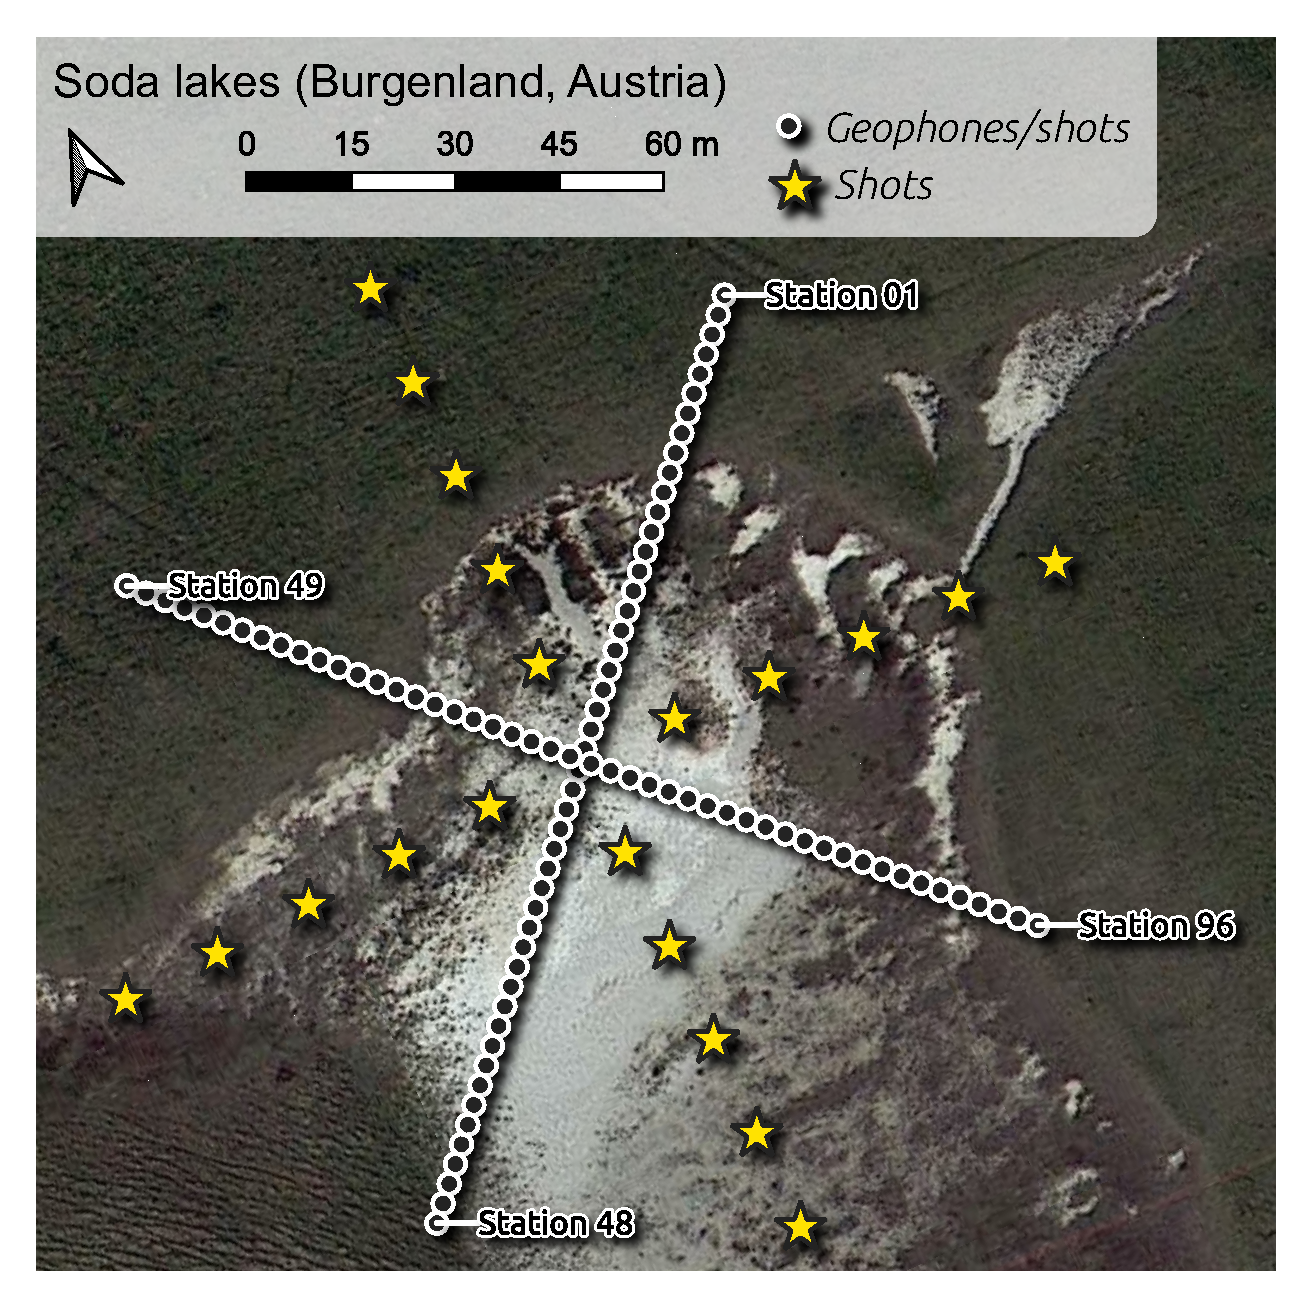
\includegraphics[width=.75\textwidth]{./figures/map_sodalakes.pdf}
	\caption{The soda lakes field dataset was collected in a 3D survey layout with stations (co-located geophones and shots indicated by filled dots) deployed in form of a cross. Additional shots (yellow stars) were conducted in from of a cross rotated by 45° to increase the coverage of the dataset.}
	\label{fig:map_sodalakes}
\end{figure}

The geometry file contains the 3D coordinates for each shot or receiver station, and thus the\\ \texttt{SeismicRefractionManager} %infers the 3D survey layout and 
automatically configures the project for 3D processing. 
Figure~\ref{fig:3d_pickwindow} presents the seismic waveform data recorded for SIN 1, i.e., the shot position co-located with the first geophone (Station 01 in Figure~\ref{fig:map_sodalakes}). The data for RIN 1 to 48 appear familiar as the corresponding SIN-RIN layout refers to the one of conventional 2D profiles; whereas the seismic waveforms for RIN 49 to 96 show an entirely different pattern. To understand such visualization, we need to take into account that RIN 49 to 96 are deployed perpendicular to the direction of propagation of the wavefront originating from SIN 1. Accordingly, the observed curvature in the first onsets is due to the varying offset of the different SIN-RIN pairs.
%Irrespective of the survey geometry, the first break traveltimes can be determined in the seismogram plot. In this particular example, the first onsets are easy to identify, thus allowing to set first break picks for almost all traces. 

\begin{figure}
	\centering
	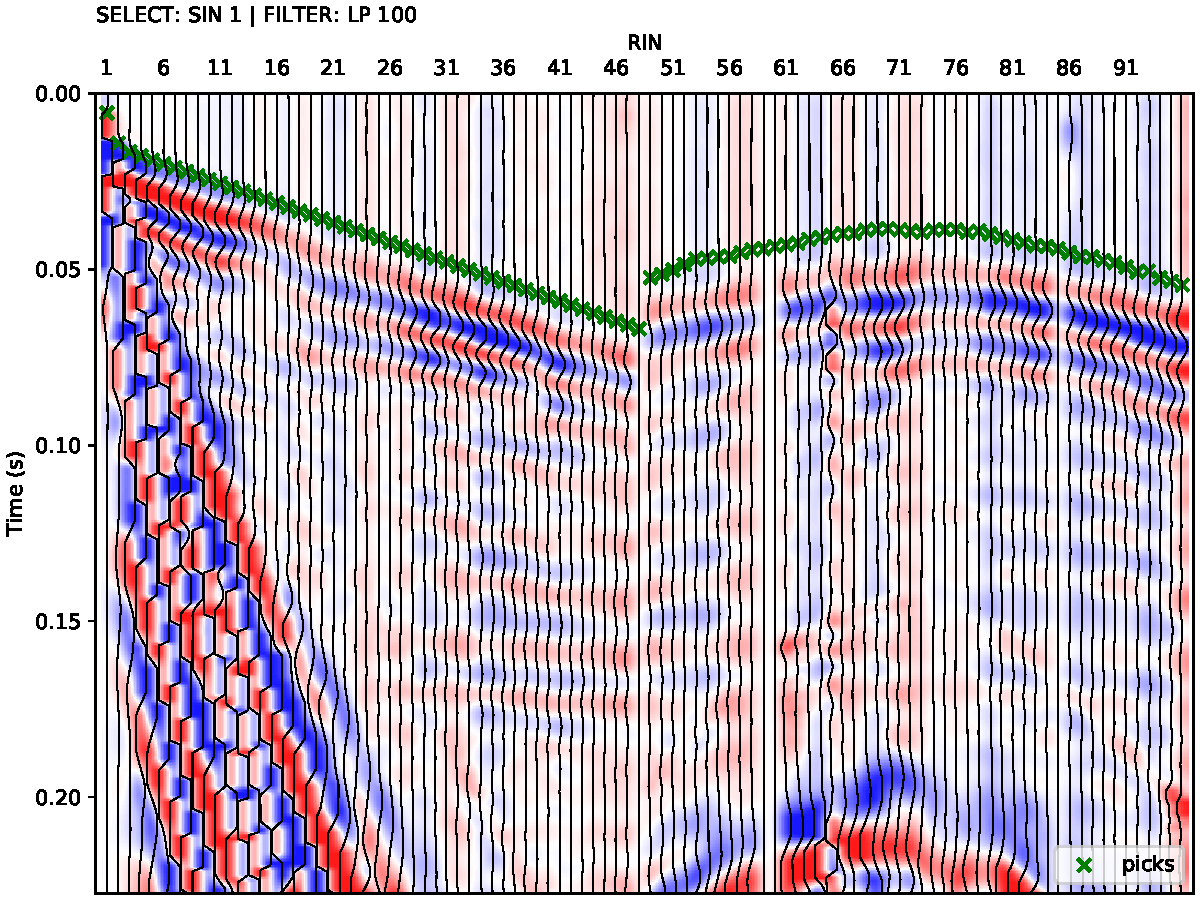
\includegraphics[width=.75\textwidth]{figures/sodalakes_sin1_lp100_picks_vd.pdf}
	\caption{Examplary seismic waveforms from the soda lakes dataset shown for shot index number (SIN) 1 with a 100 Hz lowpass filter applied to suppress high frequency noise. The recorded seismic waveforms clearly reflect the geometry of the geophones with RIN 1 to 48 deployed along the direction of wave propagation, while RIN 49 to 96 are deployed perpendicular to the propagating wavefront.}
	\label{fig:3d_pickwindow}
\end{figure}

Due to the 3D survey geometry, a 2D pseudosection is not suitable 
%we cannot use the conventional pseudosection 
to illustrate the apparent velocity values obtained from the picked first break traveltimes. Hence, 
%However, the project is configured for 3D processing so 
the \texttt{SeismicRefractionManager} automatically switches to a 3D representation where the apparent velocity values are illustrated in an interactive 3D pseudosection. This plot can be rotated and the image section can be zoomed and panned allowing the user to easily investigate the data quality for 3D geometries. Figure~\ref{fig:3d_pseudosection} shows a screenshot of the 3D pseudosection for the salt lake dataset; yet, such screenshot cannot reveal the full capabilities implemented in the \texttt{SeismicRefractionManger} for the interactive analysis and visualization of 3D pseudosections.

\begin{figure}
	\centering
	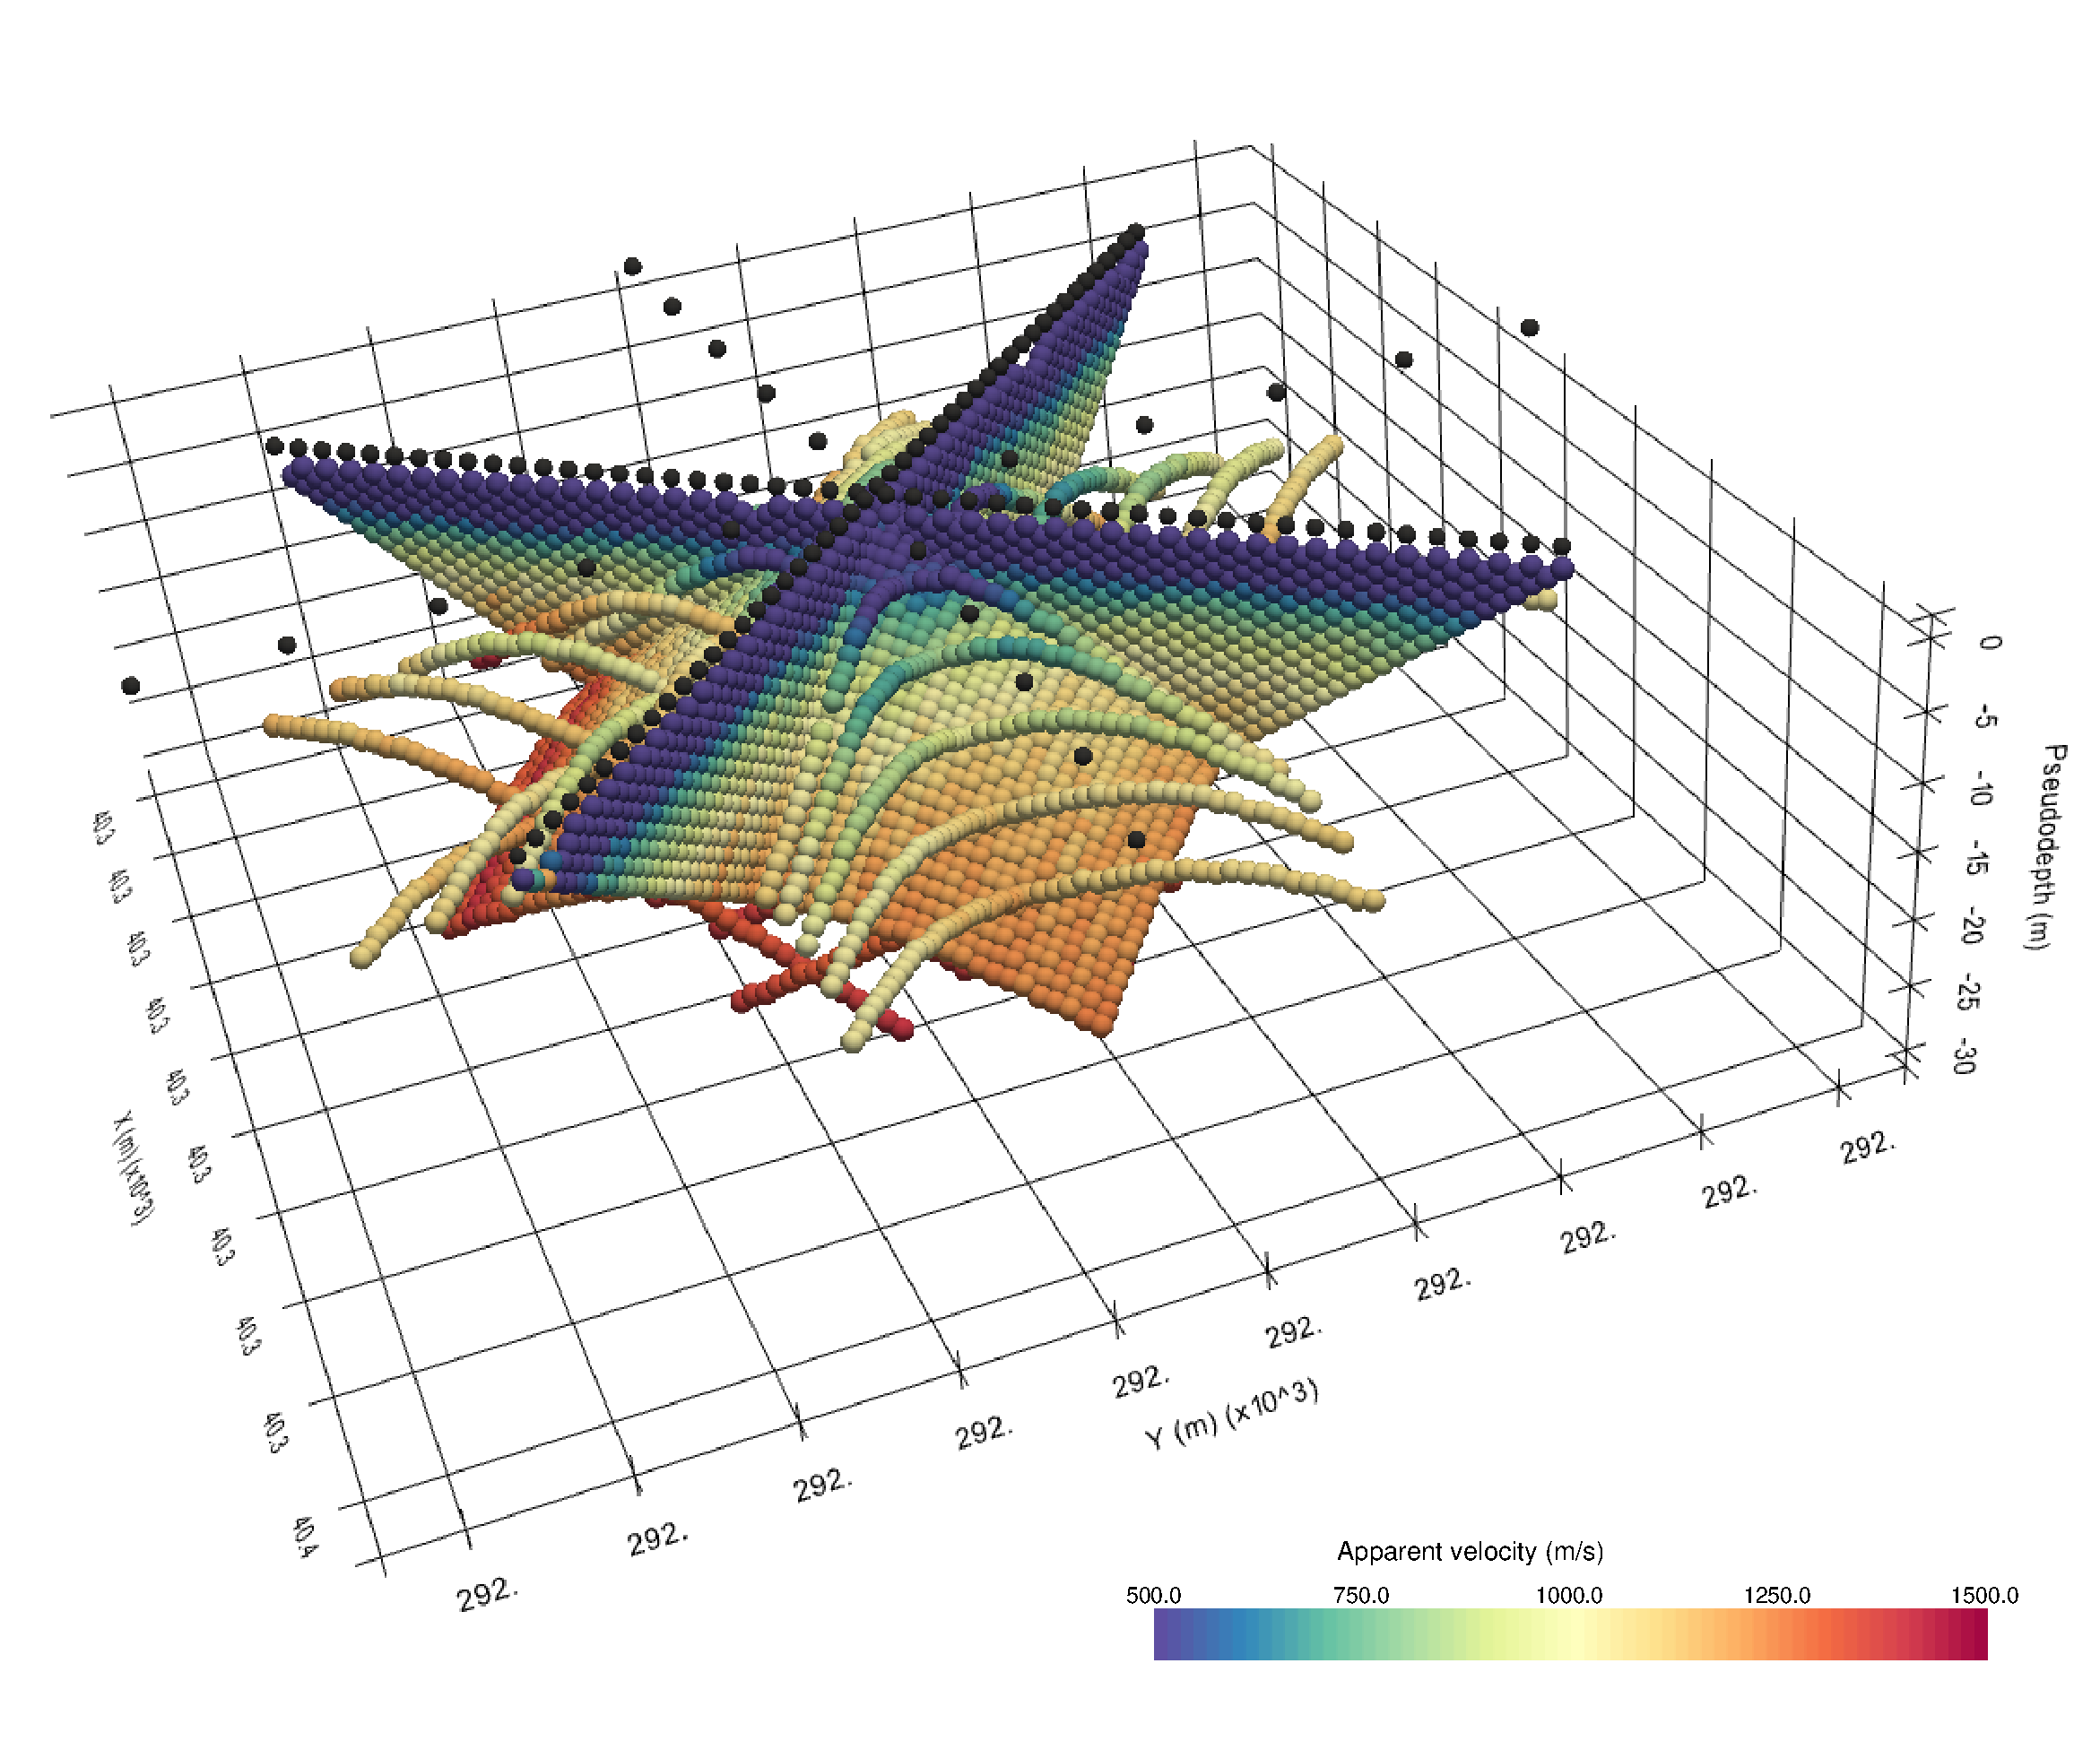
\includegraphics[width=.75\textwidth]{figures/3d_pseudosection.pdf}
	\caption{3D pseudosection showing the apparent seismic velocities determined from the first break traveltimes obtained from the soda lakes dataset and the corresponding absolute offset between the shot and receiver stations. The apparent velocity for each shot-receiver pair is illustrated at the corresponding 2D midpoint and pseudodepth (1/3 of the absolute offset), thus yielding a 3D representation.}
	\label{fig:3d_pseudosection}
\end{figure}

Once the first break picking is finished, the corresponding pickset can be exported for the inversion.
%Prior to the exporting of the first break traveltimes, it is advisable to have a look at the picking percentage to check for any missing data. As can be seen from Figure~\ref{fig:3d_pickperc}, the visualization of the picking percentage plot does not change due to the 3D survey, and thus can be read in the same way as in case of a 2D survey geometry.
The inversion results and their interpretation are not the scope of this manuscript, yet Figures~\ref{fig:3d_pickwindow} and \ref{fig:3d_pseudosection} reveal the capabilities provided by the proposed framework for the visualization and processing of data collected in 3D survey geometries.

%\begin{figure}
%	\centering
%	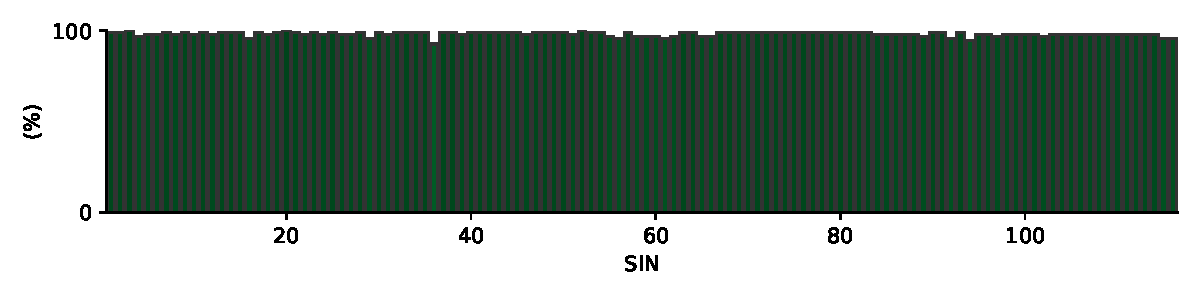
\includegraphics[width=.75\textwidth]{figures/3d_pickperc.pdf}
%	\caption{Picking percentage for each shot in the soda lakes dataset indicating a high signal-to-noise ratio allowing for the picking of first break traveltimes for nearly all shot-receiver pairs.}
%	\label{fig:3d_pickperc}
%\end{figure}

\section{Conclusions and Outlook}

We have presented formikoj, a flexible open-source library enabling the development of modeling and processing tools for geophysical data. Implemented in python and tested on all major operating systems (Linux/Unix, MacOS, Windows), formikoj is suitable for multi- and cross-platform applications; thus, allowing collaboration between users free from licensing costs and platform requirements.

We demonstrated the capabilities of the formikoj framework to develop versatile and easily scalable classes for the modeling and processing of waveforms in seismic refraction surveys. The required interaction with the user is reduced to a minimum as crucial processing steps are automatized within the \texttt{SeismicWaveformModeler} and \texttt{SeismicRefractionManager} based on efficient data input strategies, for instance the preparation and import of the geometry file or the keyboard-based interaction related to the first break picking. In this regard, the user controls the formikoj library by providing text-based commands preferably through an ipython shell to exploit the full interactive potential modeling and processing tools. However, applications of the formikoj library can also be automatized by implementing workflows in python scripts or jupyter notebooks.

Based on three exemplary use cases, we illustrated the applicability of both the \texttt{SeismicWaveformModeler} and the \texttt{SeismicRefractionManager}. In the first use case, we showed the possibility to forward model seismic waveform data based on custom subsurface models and survey geometries with the \texttt{SeismicWaveformModeler}. Additionally, the resulting waveforms can be subjected to systematic and random noise sources. 
The capabilities of the \texttt{SeismicRefractionManager} were demonstrated through the processing of field datasets collected in complex survey layout, namely a roll-along and a 3D geometry. 
Moreover, we showed how the different data visualization options can assist during the data processing to ensure consistency in the first break traveltimes. In particular, we developed a visualization of the traveltimes by means of pseuodsections illustrating the corresponding apparent seismic velocities. Such plots allow for a quick identification of systematic errors and outliers in both 2D and 3D datasets.

By making the source code of the formikoj library available under the MIT license we intend to spark the development of further modeling and processing tools for various geophysical models based on this framework. Our further efforts will focus on implementing tools for other wave-based geophysical methods used in frame of our research activities, such as multi-channel analysis of (seismic) surface waves or magnetotelluric surveys. 

\section{Acknowledgments}

%The authors acknowledge TU Wien Bibliothek for financial support through its Open Access Funding Programme.
The authors are grateful to Nathalie Roser and Lukas Aigner for benchmarking the formikoj library against established software packages in frame of their research activities. Furthermore, we would like to thank Clemens Moser, Martin Mayr, Vinzenz Schichl and Harald Pammer for their constructive comments during first tests of the formikoj framework as well as for their help during the seismic surveys.

\newpage

\textbf{Code and data availability section}

Name of the code/library: formikoj

Contact: matthias.steiner@geo.tuwien.ac.at

Hardware requirements: No specific requirements

Program language: Python
 
Software required: Anaconda/Miniconda recommended

Total program and dataset size: 250 MB

The source codes and exemplary data sets are available for downloading at the link:

https://git.geo.tuwien.ac.at/msteine1/formikoj.git

The orthophotos used in Figures~\ref{fig:map_danube} and \ref{fig:map_sodalakes} were published by geoland.at under a CC BY 4.0 license.

\bibliographystyle{cas-model2-names}
\bibliography{references} 

\end{document}

